\chapter{Complejidad y Estructuras de Datos}

\section{Complejidad}
\subsection{Notaci\'on asint\'otica}

Las notaciones que usamos para describir la complejidad temporal asint\'otica de un algoritmo est\'an definidos en t\'erminos de funciones cuyos dominios son el conjunto de los n\'umeros naturales $N = \{0,1,2,...\}$. Estas notaciones son convenientes para describir el tiempo en el peor caso de una funci\'on $T(n)$, la cual usualmente esta definida solo en tama\~nos de entrada enteros. Sin embargo a veces encontramos conveniente abusar de la notaci\'on asint\'otica en variadas formas. De todas formas, deberemos cerciorarnos de entender precisamente el significado de la notaci\'on, para que cuando hagamos abuso de la misma no estemos us\'andola de forma err\'onea. Usaremos la notaci\'on asint\'otica primariamente para describir los tiempos que insumen los algoritmos, sin embargo la notaci\'on asint\'otica aplica a funciones.

\subsubsection{Conjunto / Notaci\'on Asint\'otica $\Theta$}

Para una funci\'on $g(n)$ dada, notaremos a $\Theta(g(n))$ como el conjunto de funciones $f(n)$ que a partir de un numero $n_0 > 0$ sus valores pueden ser acotados entre $c_1g(n)$ y $c_2g(n)$ para alg\'un $c_1, c_2 \in \Re_{>0}$. Descripto formalmente quedar\'ia de la siguiente manera:

\begin{equation*}
 \Theta(g(n)) = \{ f(n) : (\exists\ c_1, c_2, n_0 \in \Re_{>0}) \ (\forall n\ |\ n_0 \leq n)\ 0 \leq c_1 \cdot g(n) \leq f(n) \leq c_2 \cdot g(n) \}
\end{equation*}

~

Una funci\'on pertenece al conjunto $\Theta(g(n))$ si existen constantes positivas $c_1$ y $c_2$ tal que $f(n)$ puede ser ``sandwicheada'' entre $c_1g(n)$ y $c_2g(n)$, para un $n$ suficientemente grande. Como $\Theta(g(n))$ es un conjunto, podremos escribir ``$f(n) \in \Theta(g(n))$'' para indicar que $f(n)$ es un miembro de $\Theta(g(n))$, a veces escribiremos ``$f(n) = \Theta(g(n))$'' para expresar exactamente lo mismo. Cuando una funci\'on $f(n)$ es acotada superiormente por otra funci\'on $c \cdot g(n)$ para alg\'un $c$ y a partir de alg\'un $n$, diremos que $f(n)$ esta \textbf{acotada asint\'oticamente} por $g(n)$ o que $f(n)$ tiene un \textbf{comportamiento asint\'otico} a $g(n)$. En el caso de $\Theta(g(n))$ diremos que $g(n)$ es una \textbf{cota asint\'oticamente ajustada} para $f(n)$.

~

\textbf{Propiedades de $\Theta$}:
\begin{enumerate}
 \item Para cualquier funci\'on $f$ se tiene que $f \in \Theta(f)$.
 \item $f \in \Theta(g) \implies \Theta(f) \subset \Theta(g)$.
 \item $\Theta(f) = \Theta(g) \iff f \in \Theta(g) \land g \in \Theta(f)$.
 \item S\'i $f \in \Theta(g) \land g \in \Theta(h) \implies f \in \Theta(h)$.
 \item S\'i $f \in \Theta(g) \land f \in \Theta(h) \implies f \in \Theta(max(g,h))$.
 \item Regla de la suma:

	S\'i $f_1 \in \Theta(g) \land f_2 \in \Theta(h) \implies f_1 + f_2 \in O(g+h)$.
 \item Regla del producto:

	S\'i $f_1 \in \Theta(g) \land f_2 \in \Theta(h) \implies f_1 * f_2 \in \Theta(g*h)$.
 \item S\'i existe $\lim_{n \to \infty} \frac{f(n)}{g(n)} = k$, seg\'un los valores que tome $k$:
	\begin{enumerate}
	  \item S\'i $k \neq 0$ y $k < \infty$ entonces $\Theta(f) = \Theta(g)$.
	  \item S\'i $k = 0$ entonces $\Theta(g) \neq \Theta(f)$.
	\end{enumerate}
\end{enumerate}

\subsubsection{Conjunto / Notaci\'on Asint\'otica $O$}

El conjunto $\Theta$ asint\'oticamente acota una funci\'on inferior y superiormente. Cuando solo tenemos una \textbf{cota asint\'otica superior}, usaremos el conjunto $O$. Para una funci\'on dada $g(n)$, denotaremos por $O(g(n))$ al conjunto de funciones tales que:

\begin{equation*}
 O(g(n)) = \{ f(n) : (\exists\ c, n_0 \in \Re_{>0}) \ (\forall n\ |\ n_0 \leq n)\ 0 \leq f(n) \leq c \cdot g(n) \}
\end{equation*}

~

Es decir que para todos los valores de $n$ a la derecha de $n_0$, el valor de la funci\'on $f(n)$ est\'a por debajo de $c \cdot g(n)$. Escribiremos $f(n) = O(g(n))$ para indicar que una funci\'on $f(n)$ es un miembro del conjunto $O(g(n))$. Notar que $f(n) = \Theta(g(n))$ implica $f(n) = O(g(n))$, ya que la noci\'on de $\Theta$ es mucho mas fuerte que la noci\'on de $O$. Esto es, escrito en forma de teor\'ia de conjuntos, que vale la inclusi\'on $\Theta(g(n)) \subseteq O(g(n))$

~

\textbf{Propiedades de $O$}:
\begin{enumerate}
 \item Para cualquier funci\'on $f$ se tiene que $f \in O(f)$.
 \item $f \in O(g) \implies O(f) \subset O(g)$.
 \item $O(f) = O(g) \iff f \in O(g) \land g \in O(f)$.
 \item S\'i $f \in O(g) \land g \in O(h) \implies f \in O(h)$.
 \item S\'i $f \in O(g) \land f \in O(h) \implies f \in O(min(g,h))$.
 \item Regla de la suma:

	S\'i $f_1 \in O(g) \land f_2 \in O(h) \implies f_1 + f_2 \in O(max(g,h))$.
 \item Regla del producto:

	S\'i $f_1 \in O(g) \land f_2 \in O(h) \implies f_1 * f_2 \in O(g*h)$.
 \item S\'i existe $\lim_{n \to \infty} \frac{f(n)}{g(n)} = k$, seg\'un los valores que tome $k$:
	\begin{enumerate}
	  \item S\'i $k \neq 0$ y $k < \infty$ entonces $O(f) = O(g)$.
	  \item S\'i $k = 0$ entonces $f \in O(g)$, es decir, $O(f) \subset O(g)$, pero sin embargo se verifica que $g \notin O(f)$.
	\end{enumerate}
\end{enumerate}

\subsubsection{Conjunto / Notaci\'on Asint\'otica $\Omega$}

De forma tal como la notaci\'on $O$ proporciona una cota asint\'otica en una funci\'on, $\Omega$ provee una \textbf{cota asint\'otica inferior}. Para una funci\'on dada $g(n)$, notaremos a $\Omega(g(n))$ como el conjunto de funciones tales que:

\begin{equation*}
 \Omega(g(n)) = \{ f(n) : (\exists\ c n_0 \in \Re_{>0}) \ (\forall n\ |\ n_0 \leq n)\ 0 \leq c \cdot g(n) \leq f(n) \}
\end{equation*}

~

Cuando decimos que el tiempo de un algoritmo es $\Omega(g(n))$, significa que no importa que particular entrada de tama\~no $n$ para cada valor de $n$, el tiempo que tardara el algoritmo con dicha entrara sera de al menos un numero constante de veces $g(n)$, para un $n$ suficientemente grande. Equivalentemente, esto nos da una cota temporal inferior para el mejor caso del algoritmo. De las definiciones de las notaciones asint\'oticas, es f\'acil ver que para cualquier dos funciones $f(n)$ y $g(n)$, tendremos que $f(n) = \Theta(g(n))$ si y solo si $f(n) = O(g(n))$ y $f(n) = \Omega(g(n))$. Usando una notaci\'on de teor\'ia de conjuntos esto seria equivalente a decir que $\Omega(g(n)) \cap O(g(n)) = \Theta(g(n))$, y si $f(n) \in \Omega(g(n)) \land f \in O(g(n))$ entonces $f(n)$ pertenecer\'a a ambos conjuntos, por lo que en particular pertenecer\'a a la intersecci\'on $\Theta(g(n))$.

~

\textbf{Propiedades de $\Omega$}:
\begin{enumerate}
 \item Para cualquier funci\'on $f$ se tiene que $f \in \Omega(f)$.
 \item $f \in \Omega(g) \implies \Omega(f) \subset O(g)$.
 \item $\Omega(f) = \Omega(g) \iff f \in \Omega(g) \land g \in \Omega(f)$.
 \item S\'i $f \in \Omega(g) \land g \in \Omega(h) \implies f \in \Omega(h)$.
 \item S\'i $f \in \Omega(g) \land f \in \Omega(h) \implies f \in \Omega(max(g,h))$.
 \item Regla de la suma:

	S\'i $f_1 \in \Omega(g) \land f_2 \in \Omega(h) \implies f_1 + f_2 \in \Omega(g+h)$.
 \item Regla del producto:

	S\'i $f_1 \in \Omega(g) \land f_2 \in \Omega(h) \implies f_1 * f_2 \in \Omega(g*h)$.
 \item S\'i existe $\lim_{n \to \infty} \frac{f(n)}{g(n)} = k$, seg\'un los valores que tome $k$:
	\begin{enumerate}
	  \item S\'i $k \neq 0$ y $k < \infty$ entonces $\Omega(f) = \Omega(g)$.
	  \item S\'i $k = 0$ entonces $g \in \Omega(f)$, es decir, $\Omega(g) \subset \Omega(f)$, pero sin embargo se verifica que $g \notin O(f)$.
	\end{enumerate}
\end{enumerate}
\subsubsection{Conjunto / Notaci\'on Asint\'otica No-Ajustada $o$}

La cota superior asint\'otica provista por $O$ puede o no puede ser ajustada asint\'oticamente, pero la cota $2n = O(n^2)$ no lo es. Usaremos la notaci\'on $o$ (o chica) para definir una cota superior que no sea ajustada asint\'oticamente. Para una funci\'on dada $g(n)$, definiremos formalmente a $o(g(n))$ como el conjunto de funciones tales que:

\begin{equation*}
 o(g(n)) = \{ f(n) : (\exists\ c, n_0 \in \Re_{>0}) \ (\forall n\ |\ n_0 \leq n)\ 0 \leq f(n) < c \cdot g(n) \}
\end{equation*}

~

Las definiciones de $O$ (o grande) y $o$ (o chica) son sumamente similares. La diferencia principal yace en que $f(n) = O(g(n))$, la cota $0 \leq f(n) \leq c \cdot g(n)$ se mantiene para alguna constante $c > 0$ mientras que en $f(n) = o(n)$, la cota $0 \leq f(n) < c \cdot g(n)$ se mantiene para todas las constantes $c > 0$. Intuitivamente, en la notaci\'on $o$, la funci\'on $f(n)$ se vuelve asint\'oticamente parecida a $g(n)$ a medida que $n$ tiende a infinito.

\subsubsection{Conjunto / Notaci\'on Asint\'otica No-Ajustada $\omega$}

Anal\'ogicamente, $\omega$ es a $\Omega$ como $o$ es a $O$. Usaremos la notaci\'on $\omega$ para referirnos a una cota inferior que no sea ajustada asint\'oticamente. Una forma de definirla en funci\'on a $o$ sera que $f(n) \in \omega(g(n))$ si y solo si $g(n) \in o(f(n))$. De todas formas formalmente definiremos a $\omega$ como el conjunto de funciones tal que dada una funci\'on $g(n)$ es:

\begin{equation*}
 \omega(g(n)) = \{ f(n) : (\exists\ c n_0 \in \Re_{>0}) \ (\forall n\ |\ n_0 \leq n)\ 0 \leq c \cdot g(n) < f(n) \}
\end{equation*}

~

A medida que $n$ tiende a infinito la relaci\'on entre $f(n)/g(n)$ se vuelve arbitrariamente grande, es decir que tiende a infinito.

\subsection{Funciones de Complejidad temporal comunes}
A continuaci\'on se listan las principales categorias de complejidad temporal, en orden creciente:
\begin{enumerate}
 \item $O(1)$ \textbf{Complejidad constante}: es independiente de los datos de entrada.
 \item $O(lg(n))$ \textbf{Complejidad logar\'itmica}: suele aparecer en determinados algoritmos con iteraci\'on o recursi\'on (por ejemplo, b\'usqueda binaria). Todos los logaritmos, sea cual sea su base, son del mismo orden, por lo que se representan en cualquier base.
 \item $O(n)$ \textbf{Complejidad lineal}: suele aparecer en bucles simples cuando la complejidad de las operaciones internas es constante o en algunos algoritmos con recursi\'on.
 \item $O(n*lg(n))$: en algunos algoritmos de ``Divide \& Conquer'' (por ejemplo, Mergesort).
 \item $O(n^2)$ \textbf{Complejidad cuadr\'atica}: aparece en bucles o recursiones doblemente anidados.
 \item $O(n^3)$ \textbf{Complejidad c\'ubica}: en bucles o recursiones triples.
 \item $O(n^k)$ \textbf{Complejidad polin\'omica} ($k \geq 1$).
 \item $O(2^n)$ \textbf{Complejidad exponencial}: suele aparecer en subprogramas recursivos que contengan dos o m\'as llamadas recursivas.
\end{enumerate}

\newpage
\section{Estructuras b\'asicas}
\subsection{Lista}
\subsection{Cola}

La estructura Cola se puede pensar como un arreglo para guardar los elementos m\'as un natural para saber la cantidad. Las colas se caracterizan por ser una estructura de tipo FIFO (First in, First out. O en castellano: Primero que entra, primero que sale).
Una implementaci\'on efectiva de una Cola puede hacerse usando \textbf{Aritmetica Circular}, alias: funci\'on m\'odulo. Idea:
\begin{enumerate}
 \item Tengo un arreglo de MAX\_CANTIDAD elementos.
 \item En una variable \textit{cant} guardo la cantidad de elementos actuales en la cola.
 \item En una variable \textit{primero} guardo la posici\'on en el arreglo del primer elemento.
 \item Encolar: agrega el nuevo elemento a la posici\'on $(primero + cant) \% MAX\_CANTIDAD$ del arreglo e  incrementa \textit{cant} en uno.
 \item Desencolar: setea $primero=(primero + 1) \% MAX\_CANTIDAD$ y decrementa \textit{cant} en uno.
\end{enumerate}
Siendo las complejidades resultantes:
\begin{itemize}
 \item \textbf{Pr\'oximo} $O(1)$
 \item \textbf{Desencolar} $O(1)$
 \item \textbf{Encolar} $O(1)$
 \item \textbf{B\'usqueda} $O(n)$
\end{itemize}
Una clara limitaci\'on de \'esta implementaci\'on es que solo puede almacenar hasta MAX\_CANTIDAD elementos al mismo tiempo. Se puede resolver esto y agregar algunas ventajas utilizando \textbf{Memoria Din\'amica}.

\subsection{Pila}
\subsection{Arreglo dimensionable}

\newpage
\section{\'Arboles}
\subsection{\'Arbol binario de b\'usqueda}

Un \'arbol binario de b\'usqueda es un \'arbol basado en nodos binarios el cual puede ser representado por una estructura de punteros en donde cada nodo es un objeto. En adici\'on a la clave y a los datos, cada nodo contiene los atributos izquierda, derecha y p, los cuales son punteros que apuntan a su hijo izquierdo, hijo derecho y padre, respectivamente. Si un hijo o un padre esta perdido el atributo apropiado contiene el valor $NIL$. El nodo ra\'iz es el \'unico nodo cuyo padre es $NIL$.

Las claves en un \'arbol binario de b\'usqueda siempre est\'an guardadas de forma tal de satisfacer la \textbf{invariante del \'arbol binario de b\'usqueda}, el cual se define como: ''Sea $x$ un nodo en un \'arbol de b\'usqueda binario. Si $y$ es un nodo en el sub-\'arbol izquierdo de $x$, entonces $y.clave \leq x.clave$. Si $y$ es un nodo en el sub-\'arbol derecho de $x$, entonces $y.clave \geq x.clave$``

\subsubsection{B\'usqueda}

La b\'usqueda en un \'arbol binario se logra utilizando el invariante presentado anteriormente. El procedimiento comienza en la ra\'iz y por cada nodo $x$ que encuentra compara la clave $k$ con $x.clave$, si las dos claves son iguales, la b\'usqueda termina. Si $k$ es mas chico que $x.clave$, la b\'usqueda continua por el sub-\'arbol izquierdo de $x$, dado que el invariante del \'arbol binario de b\'usqueda implica que $k$ no puede ser guardado en el sub-\'arbol derecho. Sim\'etricamente, si $k$ es mas grande que $x.clave$, la b\'usqueda continua por el sub-\'arbol derecho. Los nodos encontrados durante la recursion forman un camino simple desde la ra\'iz, por lo que el tiempo de corrida de una b\'usqueda en un \'arbol binario es de $O(h)$, en donde $h$ es la altura del \'arbol la cual puede ser $n$ si tenemos un \'arbol totalmente degenerado, que de cierta forma terminar\'ia siendo una lista enlazada.

Adem\'as, siempre podremos encontrar un elemento en un \'arbol binario cuya clave sea un m\'inimo o un m\'aximo siguiendo los punteros izquierdos o derechos desde la ra\'iz hasta que encontremos un $NIL$.

\subsubsection{Inserci\'on}

Las operaciones de inserci\'on y borrado causa que la din\'amica del conjunto representado por un \'arbol binario de b\'usqueda cambie. La estructura de datos debe ser modificada para reflejar este cambio, pero de forma tal que el invariante se conserve.

Para insertar un nuevo valor $v$ en un \'arbol binario de b\'usqueda $T$, crearemos un nuevo nodo $z$ de tal forma que $z.clave = v$, $z.izq = NIL$ y $z.der = NIL$. Modificara $T$ y alguno de los atributos de $z$ de tal forma que inserte $z$ en la posici\'on apropiada del \'arbol. Para lograr insertar el nuevo nodo el procedimiento guardar\'a en una variable $p$ un puntero al nodo actual en donde se encuentra mientras que ejecuta una b\'usqueda en el \'arbol. Una vez que llega a un nodo NIL durante la b\'usqueda, asigna $z.p = p$ y compara $z.clave$ con $p.clave$, si es mayor asigna $p.izq = z$ y si es menor $p.der = z$, de esta forma el invariante queda restaurado. El tiempo de esta operaci\'on se encontrara en el orden de $O(h)$, siendo que $h$ puede ser $n$ en el peor caso el tiempo ser\'a de $O(n)$, sin embargo el caso promedio suponiendo una distribuci\'on uniforme en la entrada de los valores sera de $O(lg(n))$.

\subsubsection{Borrado}

La estrategia general para eliminar un nodo $z$ de un \'arbol binario de b\'usqueda $T$ tiene $3$ casos b\'asicos, pero como veremos uno de ellos es algo enga\~noso.

\begin{itemize}
 \item Si $z$ no tiene hijos, entonces simplemente lo removeremos modificando su padre $z.p$ reemplazando el puntero a $z$ por $NIL$.
 \item Si $z$ solo tiene un hijo, entonces \textbf{elevaremos} dicho hijo para tomar la posici\'on de $z$ modificando el padre $z.p$ reemplazando el puntero a $z$ por el puntero al \'unico hijo de $z$.
 \item Si $z$ tiene dos hijos, entonces encontraremos el m\'inimo $y$ en el sub-\'arbol derecho de $z$ (es decir, su sucesor), para tomar la posici\'on de $z$ en el \'arbol. Como $y$ era el m\'inimo del sub-\'arbol derecho de $z$, $y.izq$ sera $NIL$ y si $y$ tiene un hijo izquierdo lo elevaremos al padre de $y$. Luego, con $y$ libre hijos, lo reemplazaremos por $z$ y le asignaremos los sub-\'arboles derecho e izquierdo, como hijos de $y$. Esto mismo se puede hacer si tomamos como $y$ el m\'aximo del sub-\'arbol izquierdo de $z$.
\end{itemize}

\subsubsection{Balanceo perfecto}

Vimos que los ABB funcionan razonablemente bien en el caso promedio, pero no dan garant\'ias. Todos los algoritmos que vimos tienen un peor caso lineal. En \'este sentido, los arreglos tambi\'en son lineales en el peor caso, pero ocupan menos memoria.

Pero si miramos en detalle, veremos que los algoritmos m\'as bien son $O(h)$, donde $h$ es la altura del \'arbol. Entonces, s\'i distribuy\'esemos los nodos del ABB de manera ``pareja'', de manera tal que el \'arbol tuviese la m\'inima altura y estuviese siempre parejo, obtendriamos unas complejidades mucho mejores.

~

\textbf{Teorema}: un \'arbol binario perfectamente balanceado de $n$ nodos (no nil, es decir $n>0$) tiene altura $\lfloor log_2 n \rfloor + 1$.

~

Supongamos que cada nodo tiene 0 o 2 hijos. Llamemos $n_i$ a la cantidad de nodos internos (m\'as la raiz) y $n_h$ a la cantidad de hojas.

~

\textit{Propiedad}: Si $n > 1$, $n_h = n_i + 1$

El caso base es trivial. $n = 3$ (raiz con dos hijos) $\implies n_h = 2 \land n_i = 1$ (la raiz). Entonces se cumple la propiedad.

Para el paso inductivo, supongamos que vale para $n_h$ y $n_i$. Ahora, agreguemos un nivel al arbol. Las hojas se duplican, $n_h' = 2n_h$ y los nodos internos crecen en tantos como antes ten\'ia hojas:
$n_i' = n_i + n_h$, por hipotesis inductiva: $n_i' = (n_h - 1) + n_h = 2n_h - 1 = n_h' - 1$. $\square$

\textit{Corolario}: al menos la mitad de los nodos son hojas.

~

Luego, sabemos que (1) $n' = n_i' + n_h'$ y (prop) s\'i $n > 1$, $n_h = n_i + 1$. Imaginemos que podamos las hojas: nos queda un \'arbol (llamemos $n$ a la cantidad de nodos) con las mismas propiedades, 1 menos de altura (llam\'emosla $h$), la mitad de los nodos y ahora todas las ramas de la misma longitud. ¿Cu\'antas veces m\'as podemos podarlo? O dicho de otra forma: ¿Cu\'antos niveles se pueden agregar desde el comienzo para tener un \'arbol de altura $h$?

Al agregar un nivel, la cantidad de nodos se duplica, porque $n_h' = n_i' + 1$, pero $n_i' = n$, entonces $n_h' = n +1$. Reemplazando en (1) nos queda que $n' = n + (n + 1) + 1$. Entonces $n = 1 $.$ 2 \dots 2 = 2^h = 2^{log_2 n}$.
Por ende, $h = log_2n$ y la altura del \'arbol era $h+1$. $\square$

~

Conclusi\'on, s\'i tuviesemos \'arboles perfectamente balanceados todas nuestras operaciones ser\'ian $O(log\ n)$. Pero mantener un balanceo perfecto es muy costoso, por lo que no es factible.
Sin embargo, podemos tener un balanceo ``casi'' perfecto, haciendo que todas las ramas tengan ``casi'' la misma longitud, donde ese ``casi'' lo vamos a interpretar de la siguiente manera: la longitud entre dos ramas cualesquiera de un nodo difiere a lo sumo en 1.

\'Esta clase de ABBs, son los llamads \'arboles AVL.

\subsubsection{Rotaciones}

Las rotaciones son operaciones locales en un \'arbol de b\'usqueda que cambian la estructura de punteros del mismo preservando el invariante del \'arbol binario, son mayormente usadas en las distintas implementaciones de \'arboles balanceados para ajustar los factores de balanceo del mismo. Usaremos dos tipos de rotaciones, rotaciones hacia la izquierda y rotaciones hacia la derecha. Cuando hacemos una rotaci\'on hacia la izquierda en un nodo $x$, asumimos que su hijo derecho $y$ no es $NIL$; $x$ podr\'a ser cualquier nodo en el \'arbol cuyo hijo derecho no es $NIL$. La rotaci\'on hacia la izquierda ''pivotea`` alrededor del enlace de $x$ a $y$ y hace a $y$ la nueva ra\'iz del sub-\'arbol, dejando como hijo izquierdo de $y$ a $x$ y trasladando a el hijo izquierdo de $y$ al lugar del hijo derecho de $x$. 

\begin{SCfigure}[1][ht!]
 \centering
 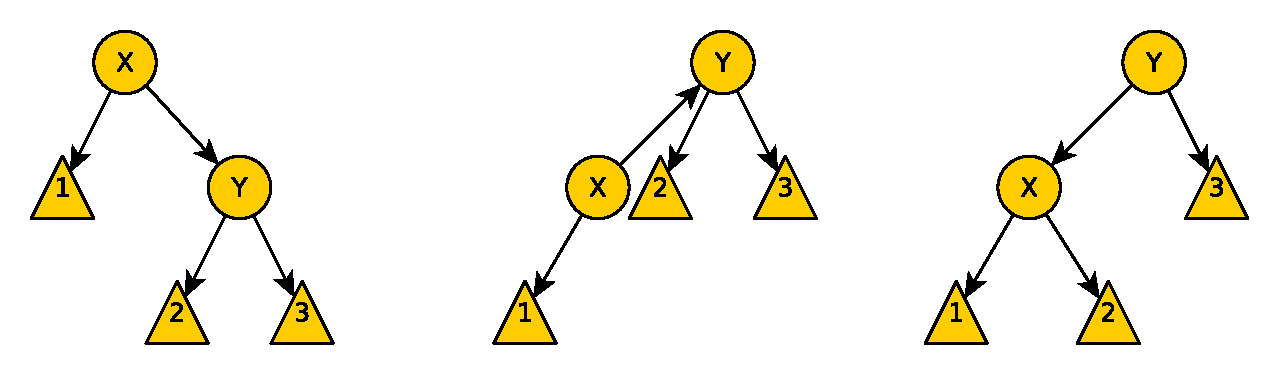
\includegraphics[width=0.7\textwidth]{graficos/RBRotacionIzq.pdf}
 \caption*{\newline \footnotesize Si nos imaginamos la rotaci\'on como bolillas e hilos, ''tirar\'iamos`` $y$ hacia arriba a la izquierda, haciendo que $x$ baje y quede a la altura del hijo izquierdo de $y$. Luego, como el hijo izquierdo de $y$ se encontraba en el sub-\'arbol derecho de $x$, sera mas grande que $x$, por lo que lo podremos asignar como hijo derecho de $x$.}
\end{SCfigure}

\subsubsection{Recorrido de \'arboles}

El recorrido de \'arboles, en ingles \textit{Tree traversal}, se refiere al proceso de visitar de manera sistem\'atica, exactamente una vez, a cada nodo de un \'arbol. Tales recorridos est\'an clasificados en el orden en el cual son visitados los nodos:

\textbf{Preorden (o ``preorder'')}: (ra\'iz, izquierdo, derecho). Comenzando con el nodo ra\'iz:
\begin{itemize}
 \item Visitar la raiz.
 \item Recorrer el sub\'arbol izquierdo en preorden.
 \item Recorrer el sub\'arbol derecho en preorden.
\end{itemize}

\textbf{Inorden (o ``inorder'')}:  (izquierdo, ra\'iz, derecho). Comenzando con el nodo ra\'iz:
\begin{itemize}
 \item Recorrer el sub\'arbol izquierdo en inordern.
 \item Visitar la raiz.
 \item Recorrer el sub\'arbol derecho en inorden.
\end{itemize}

\textbf{Postorden (o ``postorder'')}:  (izquierdo, derecho, ra\'iz). Comenzando con el nodo ra\'iz:
\begin{itemize}
 \item Recorrer el sub\'arbol izquierdo en preorden.
 \item Recorrer el sub\'arbol derecho en preorden.
 \item Visitar la raiz.
\end{itemize}

\subsubsection{Complejidades}

\begin{itemize}
 \item \textbf{B\'usqueda} $O(n)$ (caso promedio $O(lg(n))$)
 \item \textbf{Inserci\'on} $O(n)$ (caso promedio $O(lg(n))$)
 \item \textbf{Borrado} $O(n)$ (caso promedio $O(lg(n))$)
 \item \textbf{Espacio} $O(n)$
\end{itemize}

\subsection{Heap}

La estructura de datos del heap (binario) es un arreglo de objetos que representa una Cola de Prioridad y que podremos ver como un \'arbol binario casi-completo. Cada nodo del \'arbol corresponde a un elemento del arreglo y el \'arbol esta completamente lleno en todos los niveles excepto en el ultimo, el cual esta lleno desde la izquierda hasta alg\'un punto. Un arreglo $A$ que representa un heap es un objeto con dos atributos, $A.lenght$ que nos dir\'a la cantidad de elementos en el arreglo y $A.heap\_size$ que representara cuantos elementos en el heap est\'an guardados en el arreglo $A$. Esto es, que a pesar que $A[1..A.length]$ contenga n\'umeros, solo los elementos en $A[1..A.heap\_size]$ (en donde $0 \leq A.heap\_size \leq A.length$) son elementos validos del heap.

~

La ra\'iz del \'arbol estar\'a situada en $A[1]$, y dado el \'indice $i$ de un nodo, f\'acilmente podremos computar los \'indices de su padre, hijo derecho e izquierdo. El c\'omputo del \'indice del padre estar\'a definido de la forma $Padre(i) = \lfloor i/2 \rfloor$, mientras que los \'indices de los hijos podr\'an ser computados de la forma $Izquierda(i) = 2i$ y $Derecha(i) = 2i+1$, en donde $i \in [1..A.heap\_size]$. Hay dos tipos de heaps binarios, max-heaps y min-heaps. En ambos casos, los valores de los nodos satisfacen el invariante del heap, el cual depende del tipo de heap con el que trabajemos. En un max-heap, el invariante del max-heap nos dice que para cada nodo $i$ que no sea la ra\'iz se debe cumplir que $A[Padre(i)] \geq A[i]$, esto es que el valor de un nodo debe ser como m\'aximo el valor de su padre. Entonces, el m\'aximo en un max-heap estar\'a guardado en la ra\'iz, y el sub-\'arbol con ra\'iz en un nodo no podr\'a contener valores mas grandes que el nodo en si mismo. Un min-heap esta 
organizado de la forma opuesta, el invariante de min-heap nos dice que para cada nodo $i$ distinto de la ra\'iz se debe cumplir $A[Padre(i)] \leq A[i]$, por lo que el elemento m\'inimo de un min-heap estar\'a en la ra\'iz.

~

Viendo el heap como un \'arbol, definiremos la altura de un nodo en un heap como el numero de aristas en el camino simple mas largo desde el nodo mismo hasta una hoja, y definiremos la altura del heap como la altura de su ra\'iz. Ya que un heap de $n$ elementos esta basado en un \'arbol binario completo, su altura pertenecer\'a a $\Theta(lg(n))$.

\subsubsection{Mantener el invariante del heap}

De aqui en mas, asumiremos que estaremos hablando de un max-heap, ya que el min-heap es an\'alogo. Para mantener el invariante del max-heap en un arreglo, llamaremos al procedimiento \textbf{Heapify}. Su entrada sera el arreglo $A$ y un \'indice $i$ del arreglo. Cuando es llamado, Heapify asume que los sub-\'arboles binarios con sus ra\'ices en $Izquierda(i)$ y $Derecha(i)$ ser\'an max-heaps, pero que $A[i]$ puede ser mas chico que que sus hijos, violando as\'i el invariante. Heapify deja que el valor en $A[i]$ ''decante`` en el max-heap, de forma tal que el sub-\'arbol con raiz en $i$ cumpla el invariante del heap y luego recursivamente se asegurara que el invariante sea cumplido en el sub-\'arbol en donde el valor $A[i]$ haya decantado.

~

Puntualmente lo que realiza Heapify es, estando situado en $i$, compara el valor con los valores de los hijos de $i$. Si ninguno de los valores de los hijos es mas grande que el valor de $i$ lo deja como esta, en el caso contrario intercambia el valor de $i$ con el valor de su hijo mas grande. Si bien en el nodo original el invariante se cumple, el invariante puede ser violado en el sub-\'arbol cuya ra\'iz fue intercambiada por lo que se realiza una llamada recursiva utilizando como $i$ el nuevo \'indice donde el valor fue intercambiado.

~

El tiempo de Heapify en un sub-\'arbol de tama\~no $n$ con su ra\'iz en un nodo $i$ sera el tiempo $\Theta(1)$ para ajustar las relaciones entre los elementos $A[i]$, $A[Izquierda(i)]$ y $A[Derecha(i)]$, mas el tiempo que tome correr Heapify en un sub-\'arbol con su ra\'iz en alguno de los hijos del nodo $i$ (asumiendo que la llamada recursiva ocurra). El peor caso ocurrir\'a cuando el nivel inferior del \'arbol se encuentre exactamente a la mitad de estar lleno, por lo que cada uno de los sub-\'arboles de los hijos tendr\'an como mucho $2n/3$ elementos. Podremos describir el tiempo de Heapify con la recurrencia $T(n) \leq T(2n/3) + \Theta(1)$. Si tuvi\'esemos $T(n) = T(2n/3) + \Theta(1)$, la recurrencia se ajusta al segundo caso del teorema maestro, por lo que $T(n) \subseteq \Theta(lg(n))$ pero como tenemos una relaci\'on de menor o igual en la recurrencia original, $T(n) \subset O(lg(n))$.

\subsubsection{Construyendo un heap (Algoritmo de Floyd)}

Podremos usar el procedimiento Heapify de forma bottom-up para convertir un arreglo $A[1..n]$, en donde $n=A.length$, en un max-heap. Los elementos en el sub-arreglo $A[\lfloor n/2\rfloor + 1 .. n]$ son todas hojas del \'arbol, y por lo tanto cada uno es un heap de $1$ elemento por el cual podremos comenzar. El procedimiento para construir un heap va por cada uno de los nodos del \'arbol restantes comenzando por el \'indice mas grande, es decir $i = \lfloor A.length/2 \rfloor .. 1$, y ejecuta Heapify en cada uno de ellos. Una cota grosera para este procedimiento es $O(nlg(n))$, ya que har\'a $n$ llamadas a Heapify. Sin embargo, una cota mas ajustada puede ser dada bas\'andonos en que la altura de un \'arbol heap de $n$ elementos tiene altura $\lfloor lg(n) \rfloor$ y como mucho $\lceil n/2^{h+1}\rceil$ nodos de cualquier altura $h$, la cual corresponder\'a con $O(n)$.

%TODO: Dar la demostracion de esto. Pagina 157 del cormen.

\subsubsection{Extraccion de m\'aximo e inserci\'on}

El m\'aximo en un max-heap sera $A[1]$, el cual una vez extra\'ido no ser\'a eliminado del arreglo sino que ser\'a intercambiado por el ultimo elemento del arreglo y luego se decrementara $A.heap\_size$ en una unidad, dejando fuera del scope al ultimo elemento del arreglo que ser\'a aquel que acabamos de extraer. El \'unico problema con esto es que estaremos rompiendo el invariante del heap, pero para solucionarlo solo nos bastara con aplicar $Heapify(A,1)$ ya que el resto de los sub-heaps seguir\'an siendo validos. Como todas las operaciones son $\Theta(1)$ exceptuando Heapify, la cual se usar\'a una sola vez, el tiempo total del algoritmo sera de $O(lg(n))$.

%TODO: Pseudocodigo de extraccion, pagina 163 del cormen

~

Para insertar un nuevo elemento incrementaremos la variable $A.heap\_size$ en una unidad y asignaremos el nuevo valor a la ultima posici\'on valida para el heap, es decir $A[heap\_size] = valor$. Luego, intercambiaremos su valor con el padre hasta que el invariante del heap se cumpla.

%TODO: Pseudocodigo de inserci\'on, pagina 164 del cormen.

\subsubsection{En resumen}

Los heaps son \'arboles balanceados en donde la clave de cada nodo es mayor o igual que la de sus hijos y en donde todo sub-\'arbol es un heap. Adicionalmente puede o no cumplir que por la forma de su implementaci\'on sea izquierdista, esto quiere decir que el \'arbol estar\'a todo lleno exceptuando su ultimo nivel, el cual se llenara de izquierda a derecha.

Su representaci\'on podr\'a estar dada por cualquier tipo de estructura para \'arboles binarios, pero si bien sera mas eficiente si se lo representa en un arreglo, pasaremos a una representaci\'on est\'atica por lo que podremos perder tiempo agrandando un arreglo. Sea un nodo $v$, la posici\'on dentro de un heap se calcula:

\begin{itemize}
 \item Si $v$ es la ra\'iz, $P(v) = 1$
 \item Si $v$ es un nodo que no es la ra\'iz, su padre $u$ sera $P(v) = \lfloor P(u)/2\rfloor$. Sea $i$ un \'indice de un nodo: $Padre(i) = \lfloor i/2\rfloor$.
 \item Si $v$ es un hijo izquierdo de $u$ $P(v) = 2P(u)$. Sea $i$ un \'indice de un nodo: $Derecho(i) = 2i$.
 \item Si $v$ es un hijo derecho de $u$ $P(v) = 2P(v)+1$. Sea $i$ un \'indice de un nodo: $Izquierdo(i) = 2i+1$.
\end{itemize}

\subsubsection{Complejidades}
Las complejidades de las operaciones del heap quedaran de la forma:

\begin{itemize}
 \item \textbf{Ver el m\'aximo o m\'inimo / Pr\'oximo} $O(1)$
 \item \textbf{Extraer el m\'aximo o m\'inimo / Desencolar} $O(lg(n))$
 \item \textbf{Ingresar nuevo elemento / Encolar} $O(lg(n))$
 \item \textbf{Construir heap a partir de arreglo / Heapify} $O(n)$
\end{itemize}

\subsection{\'Arbol balanceado en altura (AVL)}

Un \'arbol AVL es un \'arbol binario de b\'usqueda que esta balanceado en altura. Esto es, que por cada nodo $x$, la altura de de los sub-\'arboles izquierdo y derecho de $x$ difieren en a lo sumo $1$. Para implementar un \'arbol AVL mantendremos un atributo extra en cada nodo $x.fdb$ que representara el factor de balanceo del nodo $x$. El factor de balanceo para un nodo $x$ se calculara de la forma $FDB(x) = altura(der(x)) - altura(izq(x))$.

\subsubsection{Inserci\'on}

La inserci\'on de un nuevo nodo en un principio se realiza de la misma manera que en un ABB normal. Luego de haber insertado el nodo se realizan dos acciones:

\begin{itemize}
 \item Se recalculan los factores de balanceo de forma bottom-up, es decir comenzando por el nodo reci\'en insertado hasta la ra\'iz. Esto funciona ya que los factores de balanceo de otros nodos que no pertenezcan a la rama del nodo reci\'en insertados no se ver\'an afectados por la inserci\'on.
 \item Si durante el recalculo aparece un factor $\pm 2$ en alguno de los pasos, habr\'a que rebalancear el nodo antes de continuar.
\end{itemize}

Durante el rebalanceo de un nodo aparecer\'an distintos casos para los cuales deberemos aplicar distintas rotaciones. La notaci\'on de cada uno de los casos va de la forma $D_1D_2$, siendo $x$ el nodo que necesitamos rebalancear $D_2$ indicar\'a el hijo de $x$ en cuyo sub-\'arbol $D_1$ fue hecha la inserci\'on del nuevo elemento. Es decir, si tenemos un caso $RL$, significa que estando parados en un nodo $x$ la inserci\'on fue hecha en el sub-\'arbol derecho del hijo izquierdo de $x$. De cierta forma la notaci\'on se traduce desde abajo hacia arriba en un \'arbol.

~

Estos casos son $LL$ y $RR$, a los cuales ser\'a suficiente con aplicarles rotaciones simples para solucionarlos y $LR$ y $RL$ a los cuales habr\'a que aplicarles una rotaci\'on para dejarlos en alguno de los casos anteriores y una segunda rotaci\'on para terminar de balancearlos. Tanto $LL$ a $RR$ y $LR$ a $RL$ son casos sim\'etricos unos de otros.

~

\begin{SCfigure}[1][ht!]
 \centering
 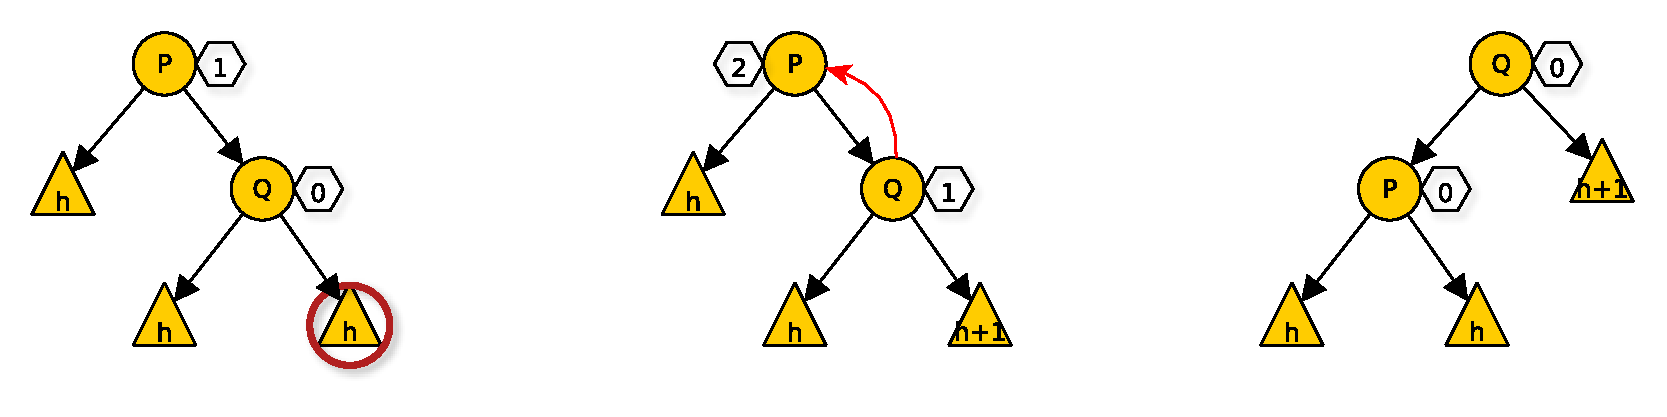
\includegraphics[width=0.70\textwidth]{graficos/RotacionSimpleAVL.pdf}
 \caption*{\newline \footnotesize \textbf{Caso RR} En la primera figura se observa el estado inicial, dentro de los hex\'agonos se encuentra el FDB de cada nodo. En la segunda figura se puede observar el estado luego de la inserci\'on y FDB desbalanceado del nodo $P$. Ejecutando una rotaci\'on hacia la izquierda entre $P$ y $Q$ se restaura, como se ve en la tercera figura (la izquierda de Q pasa a ser P, y lo que era la izquierda original de Q ahora es la derecha de P). El caso $LL$ es sim\'etrico a este caso.}
\end{SCfigure}

\newpage
\begin{SCfigure}[1][ht!]
 \centering
 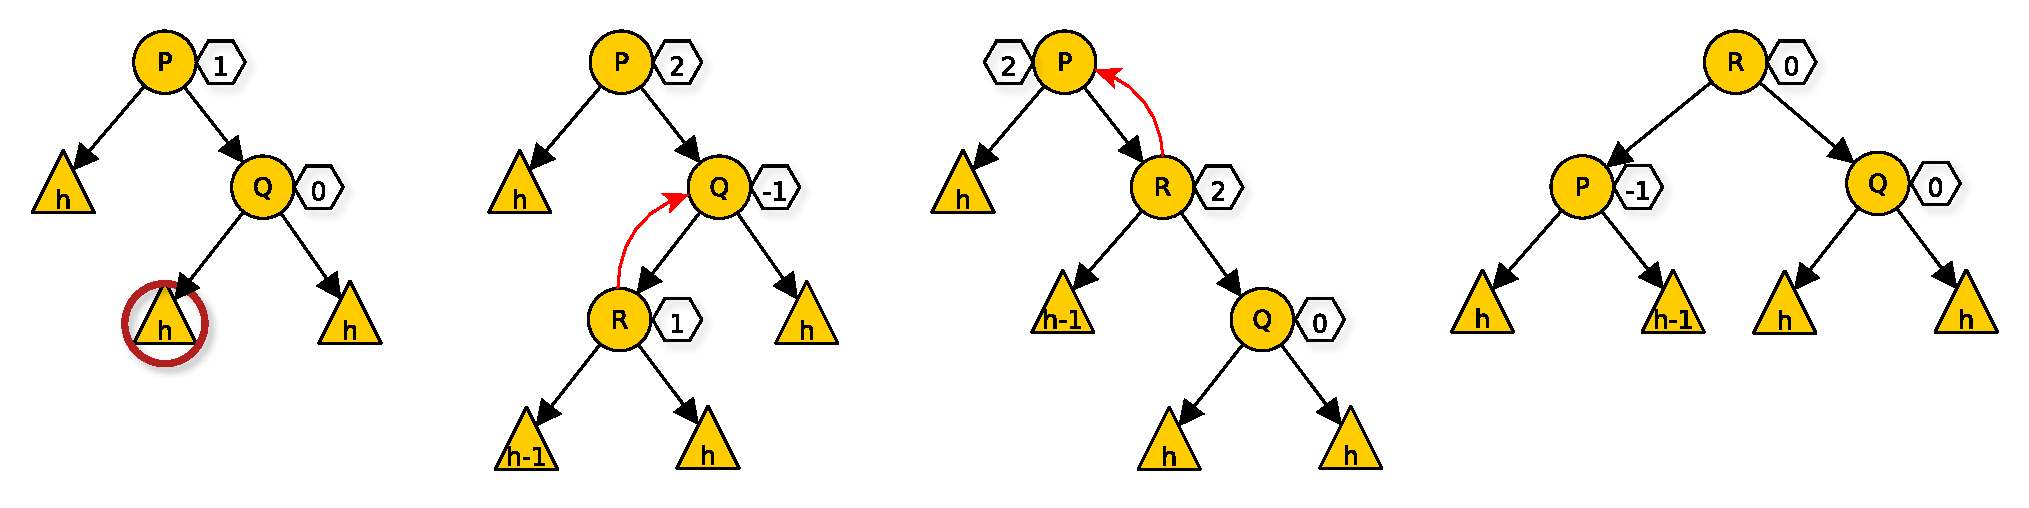
\includegraphics[width=0.70\textwidth]{graficos/RotacionDobleAVL.pdf}
 \caption*{\newline \footnotesize \textbf{Caso LR} En la primera figura se observa el estado inicial. En la segunda figura se puede observar el estado luego de la inserci\'on con el hijo izquierdo $R$ de $Q$ expandido, la primera rotaci\'on se ejecutar\'a hacia la derecha entre $R$ y $Q$. La tercer figura refleja el estado luego de la primer rotaci\'on, en este estado se ejecutara la segunda rotaci\'on que ser\'a hacia la izquierda entre $P$ y $R$. La cuarta figura refleja el estado final con el nodo balanceado. El caso $RL$ es sim\'etrico a este caso.}
\end{SCfigure}

~

La rotaciones en el caso de inserci\'on no influyen en los antepasados de $x$, por lo que su balance no ser\'a modificado, y por lo tanto a lo sumo necesitaremos realizar dos rotaciones para rebalancear el \'arbol luego de una inserci\'on. El tiempo que tomara entonces una inserci\'on sera $O(2lg(n)) \subseteq O(lg(n))$, ya que deberemos buscar el lugar para insertar el nodo y luego recalcular todos los factores de balanceo de la rama (de ser necesario se rebalancear\'a alguno de los nodos).

\subsubsection{Eliminaci\'on}

El borrado en un AVL en un principio se realiza de la misma forma que en un \'arbol binario, luego de haberlo hecho se ejecuta un recalculo de los factores y un rebalanceo sobre la rama que se vio afectada por el mismo. Una diferencia importante entre la inserci\'on y el borrado es que a la hora de realizar los rebalanceos en la inserci\'on los antepasados de un nodo $x$ desbalanceado no se ver\'an influenciados mientras que durante un rebalanceo luego de un borrado si lo har\'an. 

~

Esto \'ultimo se debe a que durante la inserci\'on estaremos agregando una hoja nueva, y por la naturaleza del AVL el balanceo de un sub-\'arbol $T$ con su raiz en $x$ ocasiona que la altura de $T$ se acorte. Esto significa que de cierta forma mediante el balanceo estaremos cancelando el incremento de altura en el sub-\'arbol $T$ ocasionado por la inserci\'on, por lo que los antepasados de $x$ no sufren modificaciones. En el caso de una eliminaci\'on, el balanceo ocasionar\'a tambi\'en que la altura del sub-\'arbol se acorte pero no habr\'a compensaci\'on por una inserci\'on, lo que decantara en una modificaci\'on de los factores de balanceo de los antepasados de $x$, pudiendo esto llegar a provocar $lg(n)$ balanceos. La complejidad de la operaci\'on de eliminaci\'on sera entonces de $O(2lg(n)) \subseteq O(lg(n))$ ya que tendremos que buscar el nodo a eliminar, actualizar los factores de balanceo y, en el peor caso, balancear toda la rama afectada (podremos actualizar los factores y rebalancear sin iterar 
nuevamente).

\subsubsection{Peor caso en eliminaci\'on}

Para lograr caracterizar un peor caso en el rebalanceo luego de la eliminaci\'on de un nodo, definiremos a $T$ como un \'arbol AVL en donde todos los nodos que no son hojas tendr\'an factor de balanceo $1$. Esto es que para todo nodo $x$ la diferencia entre la altura del sub-\'arbol derecho y el sub-\'arbol izquierdo sera $1$, es decir que $FDB(x) = altura(der(x))-altura(izq(x)) = 1$. Luego, si removemos una hoja $y$ del sub-\'arbol $izq(x)$, sea $z$ el padre de $y$ tal que $izq(z)=y$ y $izq(y) = NIL$, ocasionara que el FDB de $z$ se incremente de $1$ a $2$, ya que abremos acortado el sub-\'arbol izquierdo de $z$ en $1$ unidad.

\begin{SCfigure}[1][ht!]
 \centering
 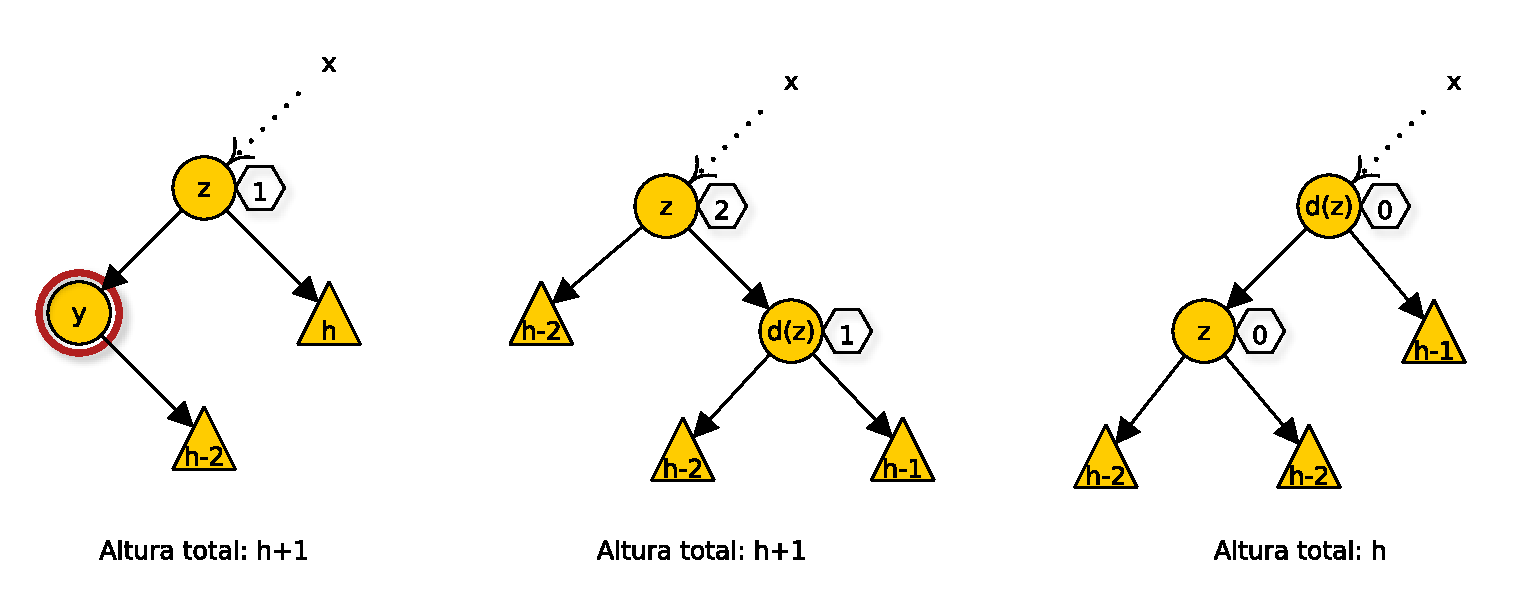
\includegraphics[width=0.70\textwidth]{graficos/PeorCasoEliminacionAVL.pdf}
 \caption*{\newline \footnotesize En la primera figura se puede apreciar el nodo $y$ a ser eliminado, junto con su padre $z$ y el FDB de $z$ en el hexagono, la altura total es de $h+1$. En la segunda figura se puede apreciar el estado luego de la eliminaci\'on del nodo $y$ junto con el hijo de derecho de $z$ expandido y los FDB correspondientes a cada nodo recalculados. Finalmente, en la tercera figura se observa el estado luego de la rotaci\'on, lo que genera un decremento en la altura del sub-\'arbol.}
\end{SCfigure}

Para compensar esto ejecutaremos una rotaci\'on hacia la izquierda entre los nodos $z$ y $der(z)$, lo que dejara a $z$ como hijo izquierdo de $der(z)$ y al hijo izquierdo de $der(z)$ como hijo derecho de $z$. Luego de la rotaci\'on los FDB de ambos nodos quedar\'an en $0$ pero la altura del \'arbol se ver\'a reducida en $1$, lo que provocar\'a que el padre original de $z$ (el abuelo de $y$), cambie su FDB de $1$ a $2$. De la misma forma deberemos continuar balanceando el resto de los nodos hasta llegar a la ra\'iz, en donde tendremos que $FDB(izq(raiz)) = 0$, $FDB(der(raiz)) = 1$ y $FDB(raiz) = 2$. Para resolver esta ultima situac\'ion podremos ejecutar una rotaci\'on hacia la derecha entre $izq(raiz)$ y $raiz$, o una rotaci\'on hacia la izquierda entre $der(raiz)$ y $raiz$. Finalmente habremos realizado exactamente $lg(alt(y))$ rotaciones, en donde $alt(y)$ es distancia a la que se encontraba $y$ de la ra\'iz, es decir su altura o nivel. Dentro de este esquema, si seleccionamos a $y$ como uno de los nodos a 
nivel $\lfloor lg(n) \rfloor$ del \'arbol, entonces tendremos el peor caso de balanceo, por lo que la complejidad de balanceo luego de una eliminaci\'on ser\'a de $O(lg(n))$.

\subsubsection{Complejidades}

\begin{itemize}
 \item \textbf{B\'usqueda} $O(lg(n))$
 \item \textbf{Inserci\'on} $O(lg(n))$
 \item \textbf{Borrado} $O(lg(n))$
 \item \textbf{Espacio} $O(n)$
\end{itemize}

\subsection{B}

Los \'arboles B son \'arboles balanceados de b\'usqueda dise\~nados para trabajar bien en discos r\'igidos u otros dispositivos de almacenamiento secundario. Los \'arboles B son similares a los \'arboles RB, pero son mejores minimizando las operaciones I/O. Varios sistemas de base de datos utilizan \'arboles B o variantes para guardar informaci\'on.

~

Los \'arboles B difieren de los \'arboles RB en el sentido de que los nodos de los \'arboles B pueden tener muchos hijos, desde unos pocos hasta miles. Esto es, que el ''factor de ramificaci\'on`` (breanching factor) de un \'arbol B puede ser bastante grande, sin embargo usualmente depende en las caracter\'isticas de la unidad de disco usada. Este tipo de \'arboles son similares a los \'arboles B en el aspecto de que cada $n-$nodo tiene altura $O(lg(n))$. La altura exacta de un \'arbol B puede ser considerablemente menos que la de un \'arbol RB por su factor de ramificaci\'on, por lo que la base del logaritmo que expresa su altura puede ser mucho mayor.

~

Los \'arboles B generalizan los \'arboles binarios en una forma natural. Si un nodo interno de un \'arbol B $x$ contiene $x.n$ claves, entonces tendr\'a $x.n+1$  hijos. Las claves en un nodo $x$ sirven como puntos de divisi\'on separando los rangos de claves manejados por $x$ en $x.n+1$ sub-rangos, cada uno manejado por un hijo de $x$. Cuando buscamos una clave en un \'arbol B, haremos una decisi\'on entre $x.n+1$ caminos basada en comparaciones con las $x.n$ claves guardadas en el nodo $x$.

~

Un \'arbol B tiene las siguientes propiedades:

\begin{enumerate}
 \item Cada nodo $x$ tiene los siguientes atributos:
 \begin{enumerate}
  \item $x.n$, el numero de claves actualmente guardadas en el nodo $x$.
  \item Las $x.n$ claves, $x.key_1, x.key_2, ..., x.key_{x.n}$, guardadas en orden creciente de forma que $x.key_1\leq x.key_2\leq ...\leq x.key_{x.n}$.
  \item $x.leaf$, un valor booleano que es verdadero si $x$ es una hoja y falso si es un nodo interno.
 \end{enumerate}
 \item Cada nodo interno $x$ adem\'as contiene $x.n+1$ punteros $x.c_1,x.c_2,...,x.c_{x.n+1}$ a sus hijos. Los nodos hojas no tienen hijos, por lo que sus atributos $c_i$ estar\'an indefinidos.
 \item Las claves $x.key_i$ separan los rangos de las claves guardadas en cada sub-\'arbol. Si $k_i$ es cualquier clave guardada en el sub-\'arbol cuya ra\'iz es $x.c_i$, entonces $k_1 \leq x.key_1 \leq k_2 \leq x.key_2 \leq ... \leq x.key_{x.n} \leq k_{x.n+1}$.
 \item Todas las hojas tienen la misma profundidad, la cual ser\'a la altura del \'arbol $h$.
 \item Los nodos tienen cotas inferiores y superiores en el numero de claves que pueden contener. Expresaremos estas cotas en terminos de un entero fijo $t \geq 2$ llamado el grado m\'inimo del \'arbol B:
 \begin{enumerate}
  \item Cada nodo distinto a la ra\'iz debe tener al menos $t-1$ claves. Cada intervalo de nodos distinto que la raiz debe tener al menos $t$ hijos. Si el \'arbol no esta vac\'io, la ra\'iz debe tener al menos una clave.
  \item Cada nodo debe contener como mucho $2t-1$ claves. Entonces, un nodo interno puede tener a lo sumo $2t$ hijos. Diremos que el nodo esta \textbf{lleno} si contiene exactamente $2t - 1$ claves.
 \end{enumerate}
\end{enumerate}

\subsubsection{Arboles 234}
El \'arbol B mas simple ocurre cuando $t=2$. Cada nodo interno puede tener 2, 3 o 4 hijos, por lo que tendremos un \'arbol $2-3-4$. En la practica, valores muchos mas grandes de $t$ nos dar\'an \'arboles B con una altura menor. Gracias a la noci\'on de cotas podremos dar una cota para la altura de un \'arbol B de la forma $h \leq log_t((n+1)/2)$, en donde $n \geq 1$, para cualquier \'arbol B de $n-$claves de altura $h$ y grado minimo $y \geq 2$.

\subsubsection{Inserci\'on en Arboles 234}

Durante la inserci\'on cada vez que encontremos un 3-nodo $x$ empujaremos al nodo del medio hacia su padre $z$ y partiremos el 2-nodo restante en dos 1-nodo. Para nodos distintos de la ra\'iz podremos hacer esto ya que el nodo $z$, por el cual ya habremos pasado, tendr\'a a lo sumo dos claves.  Si es la ra\'iz en la que nos encontramos, crearemos una nueva ra\'iz a la que podamos pasar la clave del medio. Es importante remarcar que los nodos se partir\'an a medida que los descubrimos, si se creo un 3-nodo a partir de la acci\'on de empujar una clave hacia su padre no haremos nada. Las razones por las cuales partimos los 3-nodos son asegurarnos de que haya lugar para la nueva clave en la hoja y para hacer lugar para cualquier clave que sea empujada hacia arriba. La \'unica forma en la que el \'arbol incrementara su profundidad es creando una nueva ra\'iz a causa de una inserci\'on.

\subsubsection{Eliminaci\'on en Arboles 234}

Para la eliminacion, en primer lugar buscaremos la clave a eliminar, si se encuentra en una hoja la eliminaremos y si es un nodo interno una vez encontrada la eliminaremos y buscaremos con la siguiente clave mas alta (que se encontrar\'a en un nodo hoja). Durante la eliminacion se traeran claves desde el padre o los hermanos de forma tal de asegurarnos de al menos tener dos claves en el nodo donde se efectuara la eliminacion (o de donde obtendremos el reemplazo), de cierta forma estaremos haciendo una estrategia inversa a la inserci\'on donde simplemente empujabamos las claves.

~

A medida que busquemos la clave a eliminar o su reemplazo, nos encontraremos en nodos que contengan solo una clave que deberemos lograr que tengan dos. Para lograr esto tendremos distintas estrategias seg\'un los posibles tres casos en donde nos encontremos:

\begin{enumerate}
 \item Intenta robar una clave de los hermanos inmediatamente adyacentes. Si alguno de sus hermanos tiene mas de una clave ejecutara una rotaci\'on para obtenerlo.
 \item Si no hay hermano adyacente al que podamos robarle una clave, robaremos una clave al padre (esto sera posible al menos que sea la raiz) y fusionaremos la misma con el hermano siguiente u anterior (dependiendo de la desigualdad) formando un 3-nodo.
 \item Si no hay hermano adyacente al que podamos robarle una clave, el padre es la ra\'iz y tiene solo una clave, entonces fusionaremos en un 3-nodo los hermanos y la ra\'iz, obteniendo as\'i un nuevo 3-nodo ra\'iz. Este sera el \'unico caso en donde la altura del \'arbol se ver\'a disminuida en una unidad.
\end{enumerate}

Mostraremos los tres casos mediante un ejemplo al cual se le remover\'a la ra\'iz.

\begin{SCfigure}[1][ht!]
 \centering
 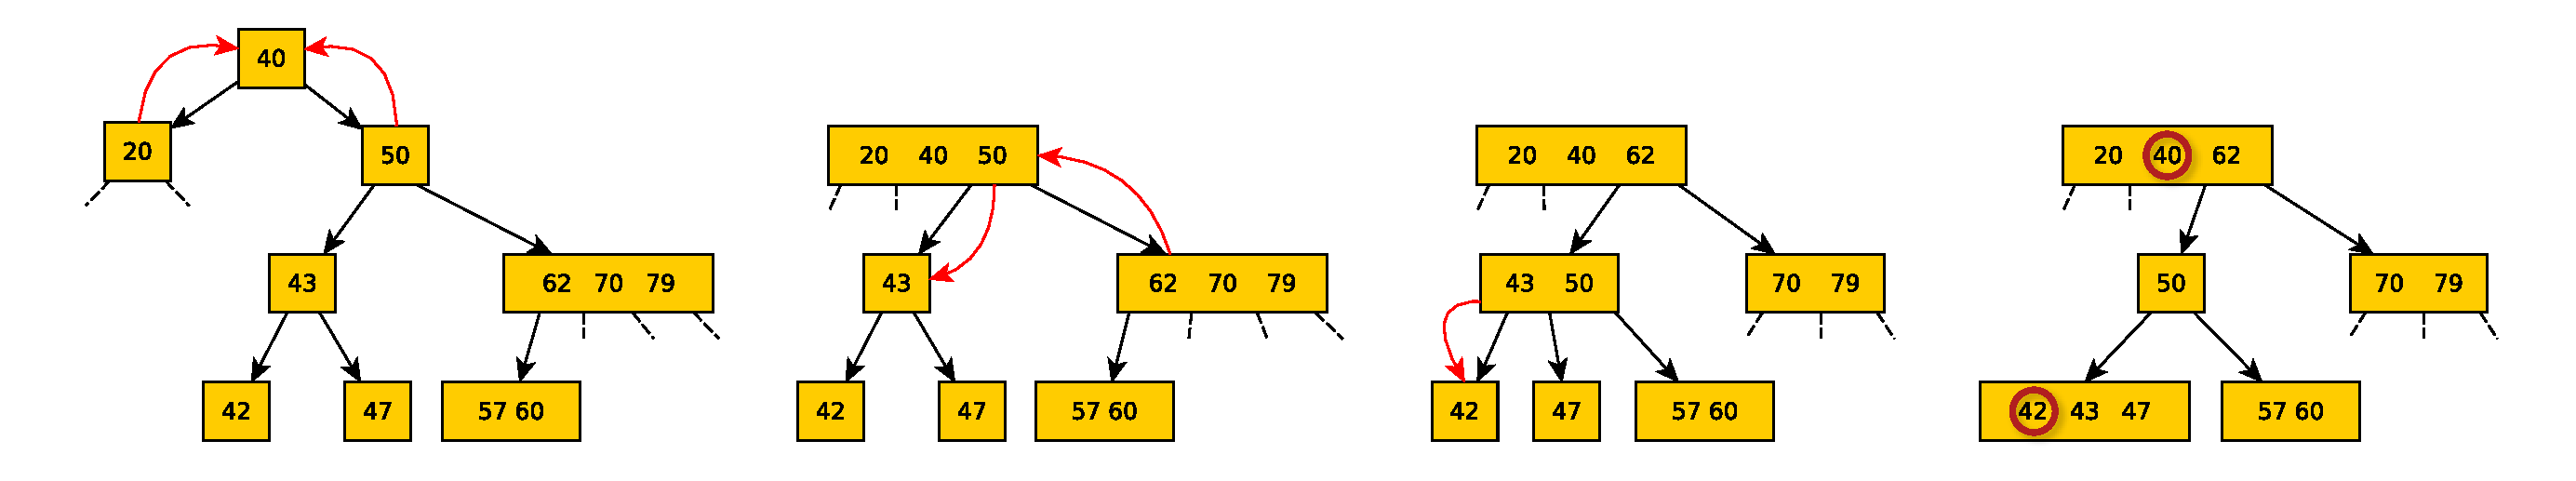
\includegraphics[width=1\textwidth]{graficos/EliminacionArboles234.pdf}
\end{SCfigure}

Como queremos remover el $40$, el objetivo sera reemplazarlo por el $42$ que se encuentra en una de las hojas del \'arbol. Una vez parados en el 1-nodo que contiene la clave $50$, veremos que aplica el tercer caso ya que el padre es la ra\'iz, y el \'unico hermano inmediato tiene solo una clave, por lo que haremos una fusi\'on como se aprecia en la segunda figura. Luego descenderemos por la rama dirigida hacia el 1-nodo que contiene el $43$, veremos que en esta instancia el primer caso es el que se ajusta, por lo cual realizaremos una rotaci\'on para terminar con un 2-nodo como se aprecia en la tercera figura. Finalmente en la tercera figura habremos descendido por el nodo que contiene a $42$ pero todav\'ia no podremos usarlo para reemplazar a $40$ ya que es un 1-nodo. En esta situaci\'on el caso que se ajustara ser\'a el segundo, ya que el \'unico hermano inmediato es el $47$, por lo que bajaremos el $43$ y lo fusionaremos con el $47$, llegando as\'i a la cuarta figura en donde podremos eliminar la clave de 
la ra\'iz y 
reemplazarlo por el $42$.

\subsection{Splay trees}

Este tipo de \'arbol tiene su inspiraci\'on en los ABB \'optimos. Los ABB \'optimos son \'arboles cuyos elementos est\'an ubicados mas cerca o lejos de la ra\'iz seg\'un la frecuencia con la que son consultados (similar a la codificaci\'on de Huffman), de esta forma optimizando los tiempos de las operaciones. El problema de este tipo de \'arboles son la rigidez, el desconocimiento de la frecuencia de las operaciones y la variabilidad que pueden sufrir estas ultimas. Los Splay Trees son ABB \'optimos aproximados que se modifican seg\'un la frecuencia de los \'ultimos elementos consultados, de esta forma mantendremos algo cercano a un ABB \'optimo que se ir\'a optimizando para los elementos que consultemos mas frecuentemente.

~

En estos \'arboles, los cuales utilizan exactamente la misma representaci\'on interna que un ABB com\'un sin ning\'un agregado, todas las operaciones toman $O(lg(n))$ en promedio. Cuando nos referimos a en promedio no nos referimos al promedio de los ABB o al Quicksort, no hay aleatorizaci\'on en los Splay Trees. De hecho, una operaci\'on simple puede tomar $\Theta(n)$ en el peor caso en donde $n$ es la cantidad de elementos en el \'arbol. Lo que podemos garantizar entonces es que cualquier secuencia de $k$ operaciones, comenzando con un \'arbol vac\'io, y con el \'arbol no creciendo mas que $>n$ elementos, entonces la secuencia a lo sumo toma $O(k\cdot lg(n))$ en el peor caso. Esto significa que podremos tener algunas pocas operaciones lentas pero la mayor\'ia ser\'an mucho mas r\'apidas, por lo que tendremos un balance en promedio de $lg(n)$ o mejor para cada operaci\'on. O dicho m\'as precisamente, los costos amortizados por operaci\'on son de $lg(n)$.

~

Otra ventaja en cuanto a otras estructuras es que los Splay Trees son mucho mas f\'aciles de programar y adem\'as otorgan acceso mas r\'apido a los datos recientemente accedidos, es decir que de cierta forma los Splay Trees tienen ''memoria`` en este aspecto. Esto \'ultimo puede darnos una performance mayor en comparaci\'on a los \'arboles 234 si tenemos un \'arbol grande y solamente accedamos algunos de los elementos ignorando la mayoria de ellos, ya que como estaremos recurriendo frecuentemente a los mismos elementos los accesos en el Splay Tree se dar\'an en $O(1)$.

~

Los Splay Trees, al igual que otros \'arboles balanceados, mantienen su balance mediante rotaciones. El balance de los Splay Trees no es perfecto, es por eso que si bien no nos garantizan una cota de $lg(n)$ en los peores casos los algoritmos utilizados para mantener cierto balance son mucho mas sencillos y r\'apidos que ene estructuras de datos balanceadas mas r\'igidamente. Adem\'as, no nos garantizaran una cota en el peor caso, pero si nos garantizan la cota en la mayor\'ia de las operaciones, lo que en la practica y para la mayor\'ia de los casos los hace igualmente buenos.

~

\subsubsection{Optimalidad de los Splay trees}
\begin{itemize}
 \item Teorema de Optimalidad Est\'atica: asint\'oticamente, los Splay Trees son tan eficientes como \textit{cualquier} ABB fijo.
 \item Teorema de Optimalidad Din\'amica: asint\'oticamente, los Splay Trees son tan eficientes como \textit{cualquier ABB que se modifique} a trav\'es de rotaciones.
\end{itemize}


\subsubsection{B\'usqueda}

Dada una clave $k$, empezaremos a buscar la clave de la misma manera que lo hacemos en un ABB hasta que encontremos la clave $k$ o hasta llegar a un $NIL$ (en el caso de que la clave no sea existente). Sea $x$ el nodo en donde la b\'usqueda termino, contenga o no $k$, elevaremos $x$ a trav\'es de una secuencia de rotaciones, de forma tal que $x$ se vuelva la ra\'iz, llamaremos a esta operaci\'on \textbf{splay}. Las razones por las cuales haremos esto ser\'an, en primer lugar, para mantener los elementos mas consultados en la ra\'iz o cerca de ella, de forma tal de que la consulta de estos sea verdaderamente r\'apida la pr\'oxima vez, y en segundo lugar, como este tipo de \'arboles puede desbalancearse (lo que es usualmente un estado temporal), si nos encontramos en un caso en donde exploremos hasta la profundidad del mismo, las rotaciones evitaran que esto pase de nuevo.

\newpage

Las rotaciones se daran en tres casos:

\begin{enumerate}
 \item \textbf{Zig-zag} $x$ es el hijo izquierdo de un hijo derecho ($LR$) o su caso espejo ($RL$). Siendo $y$ el padre de $x$ y $z$ su abuelo, para resolver este caso haremos una rotaci\'on hacia la izquierda entre $y$ y $x$ y luego una rotaci\'on hacia la derecha entre $x$ y $z$. En el caso espejo realizaremos una rotaci\'on hacia la derecha y luego una hacia la izquierda, dejando a $x$ como la raiz del sub-\'arbol.
 
 \begin{SCfigure}[1][ht!]
 \centering
 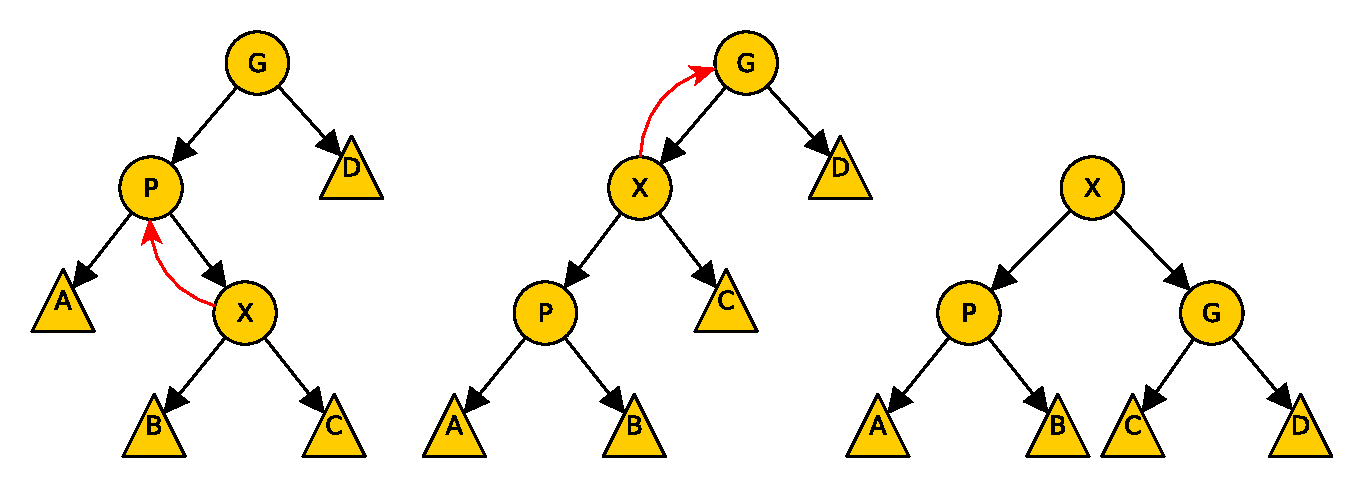
\includegraphics[width=0.5\textwidth]{graficos/ZigZagSplay.pdf}
 \end{SCfigure}
 
 \item \textbf{Zig-zig} Este caso tiene una diferencia muy sutil con el caso anterior. Si $x$ es el hijo izquierdo de un hizo izquierdo ($LL$) o su caso espejo ($RR$). Siendo $y$ el padre de $x$ y $z$ su abuelo, para resolver este caso haremos primero una rotaci\'on entre $y$ y $z$ hacia la derecha, y luego ejecutaremos otra rotaci\'on hacia la derecha entre $x$ e $y$, dejando a $x$ como la ra\'iz del sub-\'arbol.
 
 \begin{SCfigure}[1][ht!]
 \centering
 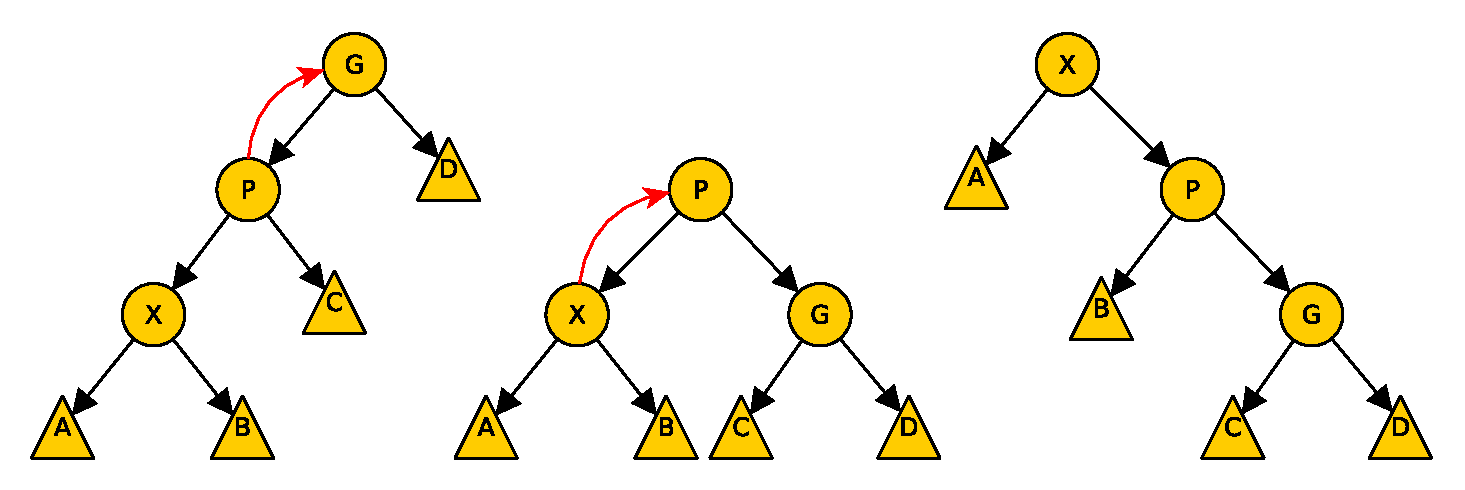
\includegraphics[width=0.5\textwidth]{graficos/ZigZigSplay.pdf}
 \end{SCfigure}
 
 ~
 
 \item \textbf{Zig} Este es un caso final que se origina al tener a $x$ a una distancia original impar de la ra\'iz en el momento del acceso. Para solucionar esto, si $x$ es el hijo izquierdo haremos una rotaci\'on hacia la derecha entre $x$ y la ra\'iz, o si $x$ es el hijo derecho haremos una rotaci\'on hacia la izquierda.
\end{enumerate}

Los casos $1$ y $2$ se repetir\'an hasta que $x$ sea la ra\'iz del \'arbol o un hijo de la ra\'iz, lo que dar\'a lugar al caso $3$. En los casos de tengamos un \'arbol totalmente degenerado hacia un lado (de forma tal que sea equivalente a una lista), la b\'usqueda nos costara tiempo $O(n)$ pero las rotaciones Zig-zig lograr\'an acortar la altura del \'arbol a la mitad, de forma tal de que las siguientes operaciones de consulta sean mucho mas eficientes. Esto ultimo se logra gracias a la forma de la rotaci\'on Zig-zig, la cual rota el abuelo y su padre antes que el hijo y su padre, si esto si hiciese en orden inverso obtendr\'iamos un \'arbol totalmente degenerado hacia la direcci\'on opuesta original. 

\subsubsection{Max/Min, Inserci\'on y Eliminaci\'on}

Las dem\'as operaciones del \'arbol usaran la operaci\'on de splay de formas similares ya que es importante para el Splay Tree ejecutar un splay cada vez que realizamos una operaci\'on sobre el mismo, ya que de esta forma el \'arbol se mantiene actualizado y balanceado segun las ultimas operaciones.

\begin{itemize}
 \item En el caso de \textbf{max/min}, una vez encontrado la max/min clave del \'arbol, haremos un splay del nodo que lo contiene.
 \item En el caso de la \textbf{inserci\'on}, una vez insertado el elemento haremos splay sobre el elemento.
 \item En el caso de la \textbf{eliminaci\'on}, una vez eliminado de la misma forma que har\'iamos en un ABB com\'un, sea $x$ el nodo eliminado del \'arbol, ejecutaremos splay sobre el padre de $x$. Si la clave que quer\'iamos eliminar no existe, aun deberemos ejecutar un splay sobre algo, por lo que lo haremos donde termino la b\'usqueda, tal como en la primera operaci\'on.
\end{itemize}

\subsection{Tries}
Los Tries son arboles (K+1)-arios para alfabetos de K elementos, o lo que es lo mismo, cada nodo puede tener a lo sumo K+1 hijos. Su nombre viene de la palabra ``Re\textbf{trie}ve''.

Motivaciones:
\begin{itemize}
 \item Tiempo menos dependiente de la cantidad de claves.
 \item Rendimiento razonable en el peor caso.
 \item R\'apidos en la pr\'actica.
 \item Adecuados para claves de tamaño variable.
\end{itemize}

La idea principal del Trie es que los ejes del \'arbol representan componentes de las claves, y cada sub\'arbol representa al conjunto de claves que comienza con las etiquetas de los ejes que llevan hasta \'el. 
De esta forma, se busca no hacer comparaciones de claves completas, sino de partes de ellas. Es decir, s\'i las claves son strings, trabajar con caracteres.

Haciendo ciertas suposiciones, la b\'usqueda o inserci\'on en un \'arbol de \textit{n} claves de \textit{b} bits necesita en promedio \textit{log n} comparaciones de clave completa, y \textit{b} en el peor caso.

~

Algunas propiedades:
\begin{itemize}
 \item La estructura del trie es la misma independientemente del orden en el que se insertan las claves.
 \item A lo sumo una comparaci\'on de clave completa (cuando llega a una hoja).
\end{itemize}

\begin{center}
 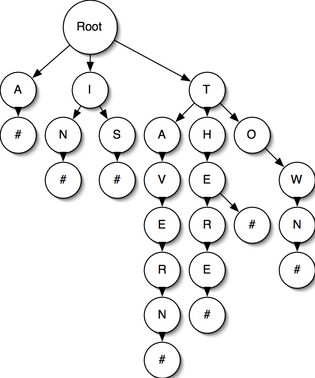
\includegraphics[width=0.25\textwidth, height=0.3\textwidth]{./graficos/trie-simple.png}
 % trie-simple.png: 315x378 pixel, 72dpi, 11.11x13.34 cm, bb=0 0 315 378
\end{center}

~

Desventajas:
\begin{itemize}
 \item Algunas implementaciones pueden requerir mucha memoria.
 \item Las operaciones sobre las componentes de las claves pueden no ser faciles, o ser muy ineficiente en algunos lenguajes de alto nivel.
\end{itemize}

\subsubsection{Tries compactos}
Consiste en colapsar las cadenas de caracteres o bits que llevan hacia hojas.
Ejemplo: en un trie con dos claves ``Algo'' y ``Algoritmos'', el camino que lleva desde la primer `o' hasta la `s' puede ser compactado en un solo nodo para ahorrar espacio.
\subsubsection{Tries Patricia}
Son Tries m\'as compactos que los mencionados anteriormente. \textit{Patricia} es un acronimo de: Practical Algorithm To Retrieve Information Coded in Alphanumeric.
La idea es colapsar todas las cadenas, no solo las que llevan a hojas (un eje ahora puede representar una cadena). 
Ejemplo: en un trie con dos claves ``Algoritmo'' y ``Algoritmos'', el camino que lleva desde el nodo `A' hasta la \'ultima `o' puede ser compactado en un solo nodo para ahorrar espacio.

\begin{center}
 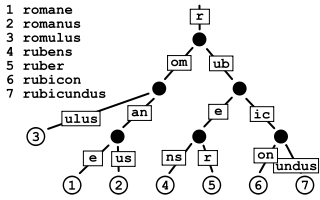
\includegraphics[width=0.4\textwidth, height=0.3\textwidth]{./graficos/trie-patricia.png}
 % trie-patricia.png: 320x200 pixel, 72dpi, 11.29x7.06 cm, bb=0 0 320 200
\end{center}

\subsection{Red-Black}

Los \'arboles RB son unos de los tantos esquemas en donde son ''balanceados`` para asegurar que las operaciones tomen $O(lg(n))$ en el peor caso. Un \'arbol RB es un \'arbol binario de b\'usqueda con un almacenamiento de un dato extra en cada nodo, su color, el cual puede ser rojo o negro. Restringiendo los colores de los nodos en cualquier camino simple desde la ra\'iz a una hoja, los \'arboles RB se aseguran que no haya camino mas largo que el doble que cualquier otro, de esta forma el \'arbol esta aproximadamente balanceado.

Cada nodo del \'arbol ahora contiene los atributos color, clave, izquierda, derecha y p. Si un hijo o el padre de un nodo no existe, el puntero correspondiente al atributo del nodo contiene el valor $NIL$. Un \'arbol RB tiene las siguientes propiedades:

\begin{enumerate}
 \item Todos los nodos son rojos o negros
 \item La ra\'iz es negra
 \item Cada hoja ($NIL$) es negra
 \item Si un nodo es rojo, entonces ambos hijos son negros.
 \item Por cada nodo, todos los caminos simples desde el nodo a hojas de descendientes tienen el mismo numero de nodos negros.
\end{enumerate}

Como conveniencia para lidiar con las condiciones borde en el c\'odigo del \'arbol RB, usaremos un \'unico centinela para presentar $NIL$. Para un \'arbol RB $T$, el centinela $T.nil$ es un objeto con los mismos atributos que cualquier otro nodo en el \'arbol. Si atributo de color es negro, y sus otros atributos tomaran valores arbitrarios. Usaremos este centinela de forma tal que podamos tratar un hijo $NIL$ de un nodo $x$ como un nodo ordinario cuyo padre es $x$. A pesar de que en cambio podr\'iamos agregar un nodo centinela distinto para cada $NIL$ en el \'arbol, de forma tal que el padre de $NIL$ este bien definido, ese enfoque nos resultara en una perdida de espacio.

Llamaremos al numero de nodos negros de un camino simple desde $x$, pero no incluy\'endolo, hasta una hoja la black-height de un nodo, denominada por $bh(x)$. Por la propiedad $5$, la noci\'on de black-height estar\'a bien definida, dado que todos los caminos simples descendientes desde el nodo tendr\'an la misma cantidad de nodos negros.

\subsubsection{Lema (cota de altura)}
Un \'arbol RB con $n$ nodos internos tiene como mucho altura $2\cdot lg(n+1)$.

~

\textbf{Prueba} Empezaremos mostrando que el sub-\'arbol con su ra\'iz en cualquier nodo $x$ contiene al menos $2^{bh(x)}-1$ nodos internos, esta sera nuestra hip\'otesis inductiva y probaremos la propiedad utilizando inducci\'on en la altura de $x$. 

Para el caso base, si la altura de $x$ es $0$, entonces $x$ debe ser una hoja ($T.nil$), y el sub-\'arbol con su ra\'iz en $x$ efectivamente contiene al menos $2^{bf(h)}-1 = 2^0 -1 = 0$ nodos internos. Para el paso inductivo, consideraremos un nodo $x$ que tiene una altura positiva y es un nodo interno con $2$ hijos (recordar que estamos considerando a los $NIL$ como hijos). Cada hijo tiene una black-height de $bh(x)$ o $bh(x)-1$, dependiendo en si su color es rojo o negro, es decir si suma o no a la black-height. Dado que la altura de un hijo de $x$ es menor que la altura de $x$ en si mismo, podremos aplicar la hip\'otesis inductiva para concluir que cada hijo tiene al menos $2^{bh(x)-1}-1$ nodos internos. Entonces, el sub-\'arbol con su ra\'iz en $x$ contiene al menos $(2^{bh(x)-1}-1) + (2^{bh(x)-1}-1) + 1 = 2^{bh(x)}-1$ nodos internos, lo que prueba la propiedad.

~

Para concluir la prueba del lema, sea $h$ la altura del \'arbol y de acuerdo con la propiedad $4$, al menos la mitad de los nodos en un camino simple desde la ra\'iz a una hoja, sin incluir la ra\'iz, deben ser negros (ya que no hay restricci\'on sobre un nodo negro con un hijo negro, y para tener la m\'inima cantidad de negros deber\'an estar alternados con rojos). En consecuencia, la black-height de la ra\'iz debe ser al menos $h/2$, entonces $n \geq 2^{h/2}-1 \implies n+1 \geq 2^{h/2}$. Si aplicamos logaritmo a ambos lados nos queda que $lg(n+1) \geq h/2 \implies h \leq 2 \cdot lg(n+1)$, lo que prueba el lema.

\subsubsection{B\'usqueda, m\'aximo y m\'inimo}

Como consecuencia directa del lema las operaci\'on de b\'usqueda, y por lo consecuente las de m\'aximo y m\'inimo, tendr\'an tiempo $O(lg(n))$ en el peor caso, en un \'arbol RB.

\subsubsection{Inserci\'on}

Podremos insertar un nodo nuevo en un \'arbol RB de $n$ nodos en tiempo $O(lg(n))$. Para lograrlo, haremos algo muy parecido a la inserci\'on del \'arbol binario de b\'usqueda. Insertaremos el nuevo nodo $z$ tal como lo har\'iamos en un \'arbol binario de b\'usqueda normal, y luego le dar\'iamos color rojo. Para garantizar que las propiedades del \'arbol RB se mantengan, realizaremos un procedimiento de reacomodaci\'on que recolorear\'a y ejecutara rotaciones sobre los nodos existentes.

~

En la inserci\'on de $z$ se mantendr\'an las propiedades $1$ y $3$, ya que no estaremos introduciendo un nuevo color y ya que $z$ tendr\'a dos hijos $NIL$ que estar\'an pintados de negro. Por lo que, las \'unicas propiedades que pueden llegar a violar ser\'an la propiedad $2$, que requiere que la ra\'iz sea negra, y la propiedad $4$, que dice que un nodo rojo no puede tener un hijo rojo. Ambas posibles violaciones son a causa de que $z$ sea pintado rojo.

~

Deberemos considerar seis casos para la reacomodaci\'on, la cual se realizara en un ciclo hasta que el \'arbol sea correcto, pero tres de los seis casos son sim\'etricos a los otros tres, por lo que realmente solamente necesitaremos considerar tres casos. Distinguiremos el caso $1$ del caso $2$ y $3$ observando el color del hermano del padre de $z$, dicho de otra forma, el t\'io de $z$. Es aqu\'i donde los $6$ casos pasan a ser $3$. Si $z.p$ es el hijo derecho, entonces el t\'io sera $z.p.p.izq$, de lo contrario sera $z.p.p.der$. Para trabajar sobre los $3$ casos distintos, haremos de cuenta que $z.p$ es el hijo izquierdo, despu\'es de todo si es el derecho solamente habr\'a que hacer un cambio de palabras. Si el color del t\'io $y$ es rojo, entonces ejecutaremos el caso $1$, de otra forma el control pasa al caso $2$ y $3$. En los $3$ casos, el abuelo $z.p.p$ es negro, dado que el padre $z.p$ es rojo, y la propiedad $4$ es solo violada entre $z$ y $z.p$.

\begin{itemize}
 \item \textbf{Caso 1: El t\'io $y$ de $z$ es rojo} Como $z.p.p$ es negro, podremos pintar $z.p$ y $y$ negros, solucionando el problema entre $z$ y $z.p$, y podremos pintar $z.p.p$ de negro par mantener la propiedad $5$. Deberemos repetir la reacomodaci\'on definiendo a $z = z.p.p$. El puntero de $z$ se mueve dos niveles mas arriba en el \'arbol.
 \item \textbf{Caso 2: El t\'io $y$ de $z$ es negro y $z$ es un hijo derecho} En este caso utilizaremos una rotaci\'on hacia la izquierda para transformar la situaci\'on en el caso $3$, en donde $z$ sera el hijo izquierdo. Dado que $z$ y $z.p$ son rojos, la rotaci\'on no afecta el black-height de los nodos o la propiedad $5$. $z$ ahora sera $z.p$.
 \item \textbf{Caso 3: El t\'io $y$ de $z$ es negro y $z$ es un hijo izquierdo} Si entramos en el caso $3$ directamente o a trav\'es del caso $2$, el t\'io $y$ de $z$ es negro, ya que de otra forma hubi\'esemos ejecutado el caso $1$. En este caso ejecutaremos una rotaci\'on hacia la derecha entre el padre $z.p$ y su abuelo $z.p.p$, lo que dejar\'a al abuelo de $z$ como hermano de $z$. Haciendo un intercambio de colores entre el padre de $z$ y el ahora hermano de $z$, lograremos restablecer la propiedad $4$ y adem\'as nos aseguramos de mantener la propiedad $5$.
 \end{itemize}

\begin{SCfigure}[1][ht!]
 \centering
 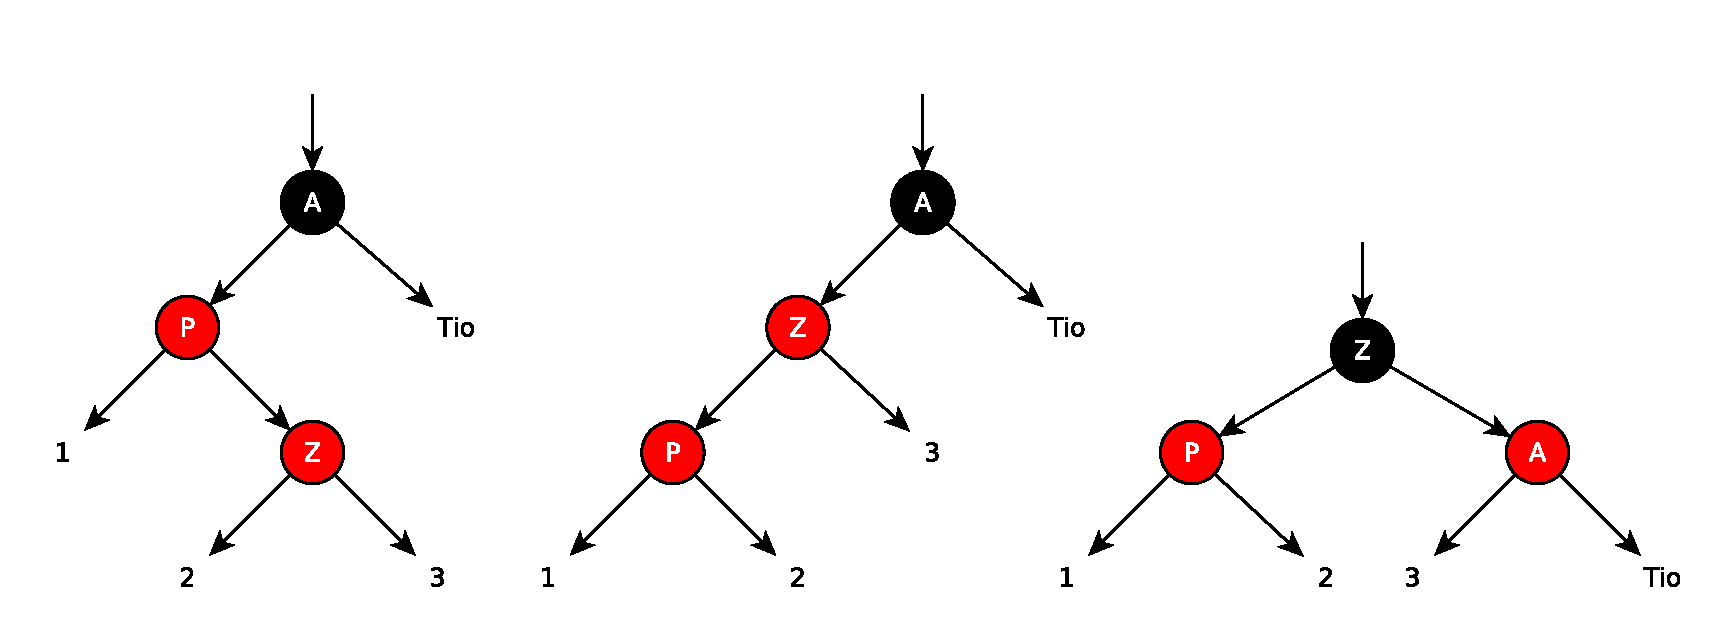
\includegraphics[width=0.75\textwidth]{graficos/RBCaso3.pdf}
 \caption*{\newline \footnotesize $z$, $p$ y $a$ representan el nodo nuevo $z$, su padre y su abuelo, respectivamente. En el primer momento estaremos en el caso $2$ y una vez ejecutada la rotaci\'on pasaremos al segundo momento. Si bien no cambiaremos los nombres por claridad, el puntero $z$ ahora estar\'a apuntando a $p$. En este momento estar\'iamos en el caso $3$, haciendo una rotaci\'on hacia la derecha mas pasar\'iamos al ultimo estado que cumplir\'a todas las propiedades.}
\end{SCfigure}
 
Dado que la altura de un \'arbol RB de $n$ nodos pertenece a $O(lg(n))$, la inserci\'on principal del nuevo nodo $z$ tomar\'a tiempo $O(lg(n))$. Cuando ejecutamos la reacomodaci\'on, solo es necesario ejecutarla nuevamente cuando ocurre el primer caso, y cuando sucede el puntero de $z$ se mueve dos niveles hacia arriba del \'arbol. Por lo tanto el numero de veces m\'aximo que deberemos ejecutar la reacomodaci\'on sera $O(lg(n))$, por lo que la inserci\'on tomar\'a en total $O(lg(n))$.

\subsubsection{Eliminaci\'on}

Eliminar un nodo de un \'arbol RB puede ser un poco mas complicado que insertar un nodo. El procedimiento para eliminar un nodo de un \'arbol RB esta basado en la eliminaci\'on del \'arbol binario de b\'usqueda.

%TODO: Falta completar esto, pagina 323 del cormen.

\subsubsection{Complejidades}

\begin{itemize}
 \item \textbf{B\'usqueda} $O(lg(n))$
 \item \textbf{Inserci\'on} $O(lg(n))$
 \item \textbf{Borrado} $O(lg(n))$
 \item \textbf{Espacio} $O(n)$
\end{itemize}

\newpage
\section{Skip lists}

Como vimos en la secci\'on de Estructuras B\'asicas, las listas son muy simples pero ineficientes. Implementar un Diccionario en dicha estructura nos dar\'ia complejidades $O(n)$ (b\'usqueda, inserci\'on y borrado).

Las Skip lists buscan tomar ventaja de esta simplicidad, pero agregando una forma de avanzar ``m\'as r\'apido'' los elementos de la lista.
En vez de que cada nodo de la lista tenga un puntero al siguiente, tendr\'an multiples punteros, dependiendo de su posici\'on en la lista, lo que nos permitir\'a dar saltos m\'as grandes a la hora de buscar/insertar un elemento.
Llevado al l\'imite, cada $2^i$-\'esimo nodo posee una referencia al nodo $2^i$ posiciones m\'as adelante en la lista:

\begin{center}
 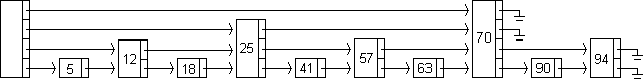
\includegraphics[width=0.75\textwidth, height=0.09\textwidth]{./graficos/skip-list-fixed.png}
\end{center}

Lo que nos da una b\'usqueda en tiempo $O(log_2(n))$ (muy similar a la b\'usqueda binaria). Notese que 1/2 de los nodos son de nivel 1, 1/4 de nivel 2, y $1/2^i$ son de nivel $2^i$.
El problema principal de \'este modelo es la rigidez en el caso din\'amico (muy dif\'icil de mantener en el caso de borrados), adem\'as de que el n\'umero total de punteros necesarios se duplica.

~

Para mejorar la idea anterior, podemos ``aleatorizar'' el requerimiento, y asignar el nivel de cada nodo probabil\'isticamente (por ejemplo, subi\'endole el nivel mientras una moneda siga saliendo ``cara'').
De \'esta forma, el costo de b\'usqueda (haciendo un an\'alisis completo) sigue siendo $O(log(n))$ en promedio (pero sin hacer hip\'otesis probabil\'isticas sobre el input). Y se pueden mejorar las constantes con una moneda cargada: $p(cara)= 1/e$

\begin{center}
 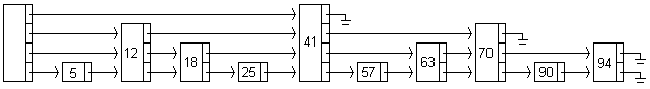
\includegraphics[width=0.75\textwidth, height=0.09\textwidth]{./graficos/skip-list-relaxed.png}
\end{center}

\subsubsection{Complejidades}

\begin{itemize}
 \item \textbf{B\'usqueda}: promedio $O(log(n))$, peor caso $O(n)$
 \item \textbf{Inserci\'on}: promedio $O(log(n))$, peor caso $O(n)$
 \item \textbf{Borrado}: promedio $O(log(n))$, peor caso $O(n)$
 \item \textbf{Espacio} promedio $O(n)$, peor caso $O(n*log(n))$
\end{itemize}

\newpage
\section{Tablas hash}

Muchas aplicaciones requieren un conjunto din\'amico que solo soporte las operaciones de diccionario inserci\'on, b\'usqueda y eliminaci\'on. Una tabla de hash es una estructura de datos efectiva para implementar diccionarios, que generaliza el concepto de arreglo. Si bien buscar un elemento en una tabla de hash puede tardar tanto como buscar un elemento en una lista enlazada ($\Theta(n)$ en el peor caso), en la practica la tabla de hash tiene una muy buena performance. Bajo suposiciones razonables, el tiempo promedio de buscar un elemento en una tabla de hash es de $O(1)$.

\subsection{Direccionamiento directo}
Se asocia a cada valor de la clave un \'indice de un arreglo. Por lo tanto, tenemos b\'usqueda, inserci\'on y borrado en $O(1)$. Por ejemplo, clave=n\'umero de DNI (n\'umero entre 0 y $10^8$).

El \'unico problema: \textbf{mucho} desperdicio de memoria.

\subsection{Conceptos b\'asicos}
Representaremos un diccionario como una tupla $\langle T,h \rangle$. Donde:
\begin{itemize}
 \item $T$ es un arreglo con $N=tam(T)$ celdas.
 \item $h: K \rightarrow\{0,\dots,N-1\}$ es la funci\'on hash (o de hash, o de hashing).
 \item $K$ conjunto de claves posibles.
 \item $\{0,\dots,N-1\}$ conjunto de las posiciones de la tabla (a veces llamadas \textit{pseudoclaves})
 \item La posici\'on del elemento en el arreglo se calcula a trav\'es de la funci\'on $h$.
\end{itemize}


Se dice que una \textbf{funci\'on de hash es perfecta} s\'i: $\forall\ k_1 \neq k_2 \implies h(k_1) \neq h(k_2)$. Y \'esto requiere $N \geq |K|$, lo que es raramente razonable en la pr\'actica, ya que en general $N < |K|$, y muy habitualmente $N < < |K|$

~

La consecuencia de esto \'ultimo es que hay \textbf{colisiones} (y son mucho m\'as frecuentes que lo intuitivo). Es decir, es posible que $h(k_1) = h(k_2)$ a\'un con $k_1 \neq k_2 $. Para resolver esto se utilizan distintos m\'etodos, que se diferencian por la forma de ubicar a los elementos que dan lugar a colisi\'on, siendo las dos familias principales:
\begin{itemize}
 \item Direccionamiento cerrado o Concatenaci\'on: a la i\-\'esima posici\'on de la tabla se le asocia la lista de los elementos tales que $h(k)=i$
 \item Direccionamiento abierto: todos los elementos se guardan en la tabla.
\end{itemize}

Llamaremos $P$ a la \textbf{distribuci\'on de probabilidad de las claves}, tal que $P(k) = $ ``probabilidad de la clave k''. Para disminuir la probabilidad de colisiones, nos gustar\'ia que los elementos se distribuyan en el arreglo de manera uniforme. O lo que es lo mismo, pedir Uniformidad Simple:
$$\forall\ j \sum_{k \in K : h(k) = j}P(k) = 1 / |N|$$

Pero es muy d\'ificil construir funciones que satisfagan Uniformidad Simple, ya que $P$ es generalmente desconocida.

\subsection{Direccionamiento cerrado o Concatenaci\'on}
A la i-\'esima posici\'on de la tabla se le asocia la lista de los elementos tales que $h(k)=i$. Por ejemplo, para una tabla de 5 celdas: $h(k) = k\ mod\ 5$

Complejidades
\begin{itemize}
 \item \textbf{B\'usqueda}: lineal en la lista asociada a la posici\'on $h(k)$: $O($longitud de la lista asocidada a $h(k))$
 \item \textbf{Inserci\'on}: al principio de la lista asociada a la posici\'on $h(k)$: $O(1)$
 \item \textbf{Borrado}: b\'usqueda en la lista asociada a la posici\'on $h(k)$: $O($longitud de la lista asocidada a $h(k))$
\end{itemize}

~

Luego, bajo la hip\'otesis de Uniformidad Simple de la funci\'on de hash, en promedio:
\begin{itemize}
\item Una b\'usqueda fallida requiere $\Theta(1+\alpha)$
\item Una b\'usqueda exitosa requiere $\Theta(1+\alpha / 2)$
\item Con $n=\#$elementos en la tabla, y $\alpha = n / |T|$ (factor de carga).
\end{itemize}

Por lo que sí $n \sim T$, obtenemos $O(1)$

\subsection{Direccionamiento abierto}
A diferencia del Direccionamiento cerrado, todos los elementos se almacenan en la tabla, y las colisiones tambi\'en se resuelven dentro de la tabla.

Ideas b\'asicas:
\begin{itemize}
\item S\'i la posici\'on calculada est\'a ocupada, hay que buscar una posici\'on libre.
\item La funci\'on de hash pasa a depender tambi\'en del n\'umero de intentos realizados para encontrar una posici\'on libre, es decir: $h(k,i)$ para el i-\'esimo intento, y $h$ debe generar todas las posiciones de $T$.
\item Los distintos m\'etodos de direccionamiento abierto se distinguen por el m\'etodo de barrido que utilizan.
\item Puede pasar que al buscar una posici\'on libre nos de \textit{overflow} (la tabla se llena y hay que borrar alg\'un elemento antes de poder insertar uno nuevo).
\end{itemize}

\subsubsection{Fen\'omenos de Aglomeraci\'on}
\begin{itemize}
\item Aglomeraci\'on primaria: s\'i dos secuencias de barrido tienen una colisi\'on, siguen colisionando, y los elementos se aglomeran por largos tramos.
Ejemplo: $h(k,i) = (h'(k) + i)\ mod\ 101$, en una lista de 101 elementos, con la secuencia de inserciones: $\{2, 103, 104, 105,\dots\}$. Los elementos se aglomeran en un solo bloque.
\item Aglomeraci\'on secundaria: s\'i dos secuencias de barrido tienen una colisi\'on en el primer intento, sigue habiendo colisiones.
\end{itemize}

\subsubsection{Barrido lineal}
Para recorrer toda la tabla usamos:
$$h(k,i) = (h'(k) + i)\ mod\ |T|$$
donde $h'(k)$ es una funci\'on de hashing. Luego, se recorren todas las posiciones en la secuencia: $T[h'(k)], T[h'(k) + 1], \dots, T[|T|], 0, 1, \dots, T[h'(k) - 1]$. Tiene posibilidad de aglomeraci\'on primaria.
\subsubsection{Barrido cuadr\'atico}
Usamos:
$$h(k,i) = (h'(k) + c_1 * i + c_2 * i^2)\ mod\ |T|$$
donde $h'(k)$ es una funci\'on de hashing, $c_1$ y $c_2$ constantes. Tiene posibilidad de aglomeraci\'on secundaria.
\subsubsection{Hashing doble}
\'Este barrido depende tambi\'en de la clave:
$$h(k,i) = (h_1(k) + i * h_2(k))\ mod\ |T|$$
donde $h_1(k)$ y $h_2(k)$ son funciones de hashing. Reduce los fen\'omenos de aglomeraci\'on secundaria, y no tiene aglomeraci\'on primaria.
\subsubsection{Hashing din\'amico o extensible}